\documentclass[10pt,twocolumn,letterpaper]{article}

\usepackage[pagenumbers]{cvpr} % To force page numbers, e.g. for an arXiv version

\usepackage{graphicx}
\usepackage{amsmath}
\usepackage{amssymb}
\usepackage{booktabs}
\usepackage[acronym]{glossaries}
\usepackage{float}

\usepackage[pagebackref,breaklinks,colorlinks]{hyperref}

\usepackage[capitalize]{cleveref}
\crefname{section}{Sec.}{Secs.}
\Crefname{section}{Section}{Sections}
\Crefname{table}{Table}{Tables}
\crefname{table}{Tab.}{Tabs.}

\def\cvprPaperID{*****}
\def\confName{CVPR}
\def\confYear{2022}

\graphicspath{ {./figures/} }
\DeclareGraphicsExtensions{.pdf,.jpg,.png}

\newacronym{svm}{SVM}{Support Vector Machine}
\newacronym{cnn}{CNN}{Convolutional Neural Network}
\newacronym{pca}{PCA}{Principal Component Analysis}


\begin{document}

\title{Star Tracker without a Star Database}

\author{Stephen Scott\\
McMaster University\\
1280 Main St W, Hamilton, ON L8S 4L8\\
{\tt\small scotts24@mcmaster.ca}
}
\maketitle

%%%%%%%%% ABSTRACT
\begin{abstract}
   A star tracker is a system used to assist a satellite in attitude estimation, which has conventionally been costly to implement and requires complex algorithms to accurately detect star patterns and subsequently calculate attitude vectors. As the popularity of nanosatellites increases, there is a growing need to simplify star tracker algorithms for implementation on university-level projects where budgets are low. In the past, star tracker algorithms have relied on star matching based on star lookup tables; however, in this paper a method is investigated to perform attitude estimation using star field images without a star database. A case study is performed on a dataset of simulated star images using the proposed approach and the results are presented.
\end{abstract}

%%%%%%%%% BODY TEXT
\section{Introduction}
\label{sec:intro}

Spacecraft attitude determination is the process by which a satellite uses sensors to estimate its orientation and is important to the satellite control problem because it provides a means for the satellite to adjust its trajectory with respect to a reference vector CITE. The popularity of nanosatellites like CubeSats is increasing, and typically these small platforms are much more limited both with respect to costs and available hardware when compared to conventional satellites. Attitude determination algorithms often use a fusion of data from multiple sensors to determine the best estimate of the satellite's orientation. The star tracker is a candidate for these applications; however, the star tracker can be a costly component to add to a low-budget spacecraft like a CubeSat CITE. Smith suggests that a star tracker can be made from budgetary hardware; however, the software to process the star tracker data in a meaningful manner is a non-trivial task and can propose a barrier to university teams developing nanosatellites. 

Star trackers often rely on lookup tables to identify stars; however, in recent years neural networks have been incorporated into the star tracker software stack CITE. The star tracker system involves an optic system used to capture light from stars. An image is developed from the optics and is typically fed through a series of algorithms including star detection and centroiding, star identification, and finally attitude estimation CITE. A crucial part of the overall algorithm is feature extraction from the star detection and centroiding. Another important aspect of the system is the onboard database which stores star features for the identification process CITE. A magnitude threshold is used to populate the database since the photodetectors can only identify stars of a certain magnitude. Also, stars that have centroids too close to one another are ignored.


\section{Related Work}
\label{sec:related}

One of the recent developments in star identification is a pattern-based feature extraction method called the correlation algorithm which compares the camera images to images in the database by maximizing a cost function. Star locations are represented as Gaussian distributions and the images are correlated with the database image in the image space to attain a heat map CITE.

Another approach to star identification that utilizes image processing is the approach presented by Delabie \etal in CITE. Similar to the method proposed by Yoon \etal CITE, the method uses image matching techniques to match pairs of images optimally on top of each other such that the stars are aligned. The advantage of this algorithm is that it eliminates the need for computationally expensive coordinate system conversions that are often present in an attitude estimation algorithm. The method uses a shortest distance transform to create a mapping of the inter-star pixel distances for which the Euclidean squared distance metric is used.

These two approaches are similar in that they rely on on-board datasets of images in order to identify stars and subsequently lookup the star coordinates in the database. This introduces an O(n) time complexity to the algorithm as the star lookup time scales linearly with the number of stars in the lookup table.




\section{Proposed Method}
\label{sec:method}

The proposed method seeks to eliminate the need for a star lookup table by directly classifying attitude vectors from input star images. To accomplish this, the algorithm must be trained using a dataset of star field images with labelled right ascension and declination values with respect to the center pixel of the image. This dataset is for usage in creating a supervised learning model ahead of the star tracker implementation, and thus the dataset is not required on-board the satellite. A limitation of this approach is that it is sensitive to the field of view of images in the dataset. Thus, for the algorithm to be useful for a particular application, the practitioner must create a dataset of images for the field of view corresponding to the camera used for the application. This field of view can be determined from the focal length of the camera CITE. Additionally, as the method is described herein, the algorithm is sufficient only for vague attitude estimation as will be described in Section \ref{sec:results}.

\subsection{Dataset Generation}

For the purpose of validating the proposed algorithm, a simulated dataset of star field images was generated using Stellarium. The dataset has been released open-source with accompanying right ascension and declination labels CITE. Stellarium is a free open-source planetarium that can be used to explore the night sky in a realistic 3D environment CITE. One of the useful features of Stellarium is that it allows the user control over the visible elements in the environment. For the purpose of this simulation, the visible elements were modified to create an environment which mimics that of a satellite in space. An assumption is made that the shutter speed of the camera is low enough such that the backdrop of the milky way and deep space objects are not visible in the images, and thus the corresponding elements are disabled in Stellarium.

After preparing the simulation environment, a Stellarium script was used to sweep through right ascension and declination angles in 5 degree increments from 0 and -90 degrees to 355 and 85 degrees, respectively. Due to this angle sweeping, the image dataset covers the full spherical field of view of the sky. At each increment, an image was captured from Stellarium and the resulting dataset has 2,592 images total. For the purpose of this investigation, the resulting images were further labelled into 4 classes representing the North-East, North-West, South-East, and South-West skies using the right ascension and declination angles. Positive declination angles are used to classify the North sky and right ascension angles less than 180 degrees are used to classify the Eastern sky. An example image from the dataset is shown in Figure \ref{fig:star_img}. This image will be used in further sections to visualize preprocessing and feature extraction steps of the algorithm.

The script used to prepare the dataset and subsequent scripts are available on GitHub CITE.

\begin{figure}[H]
  \centering
   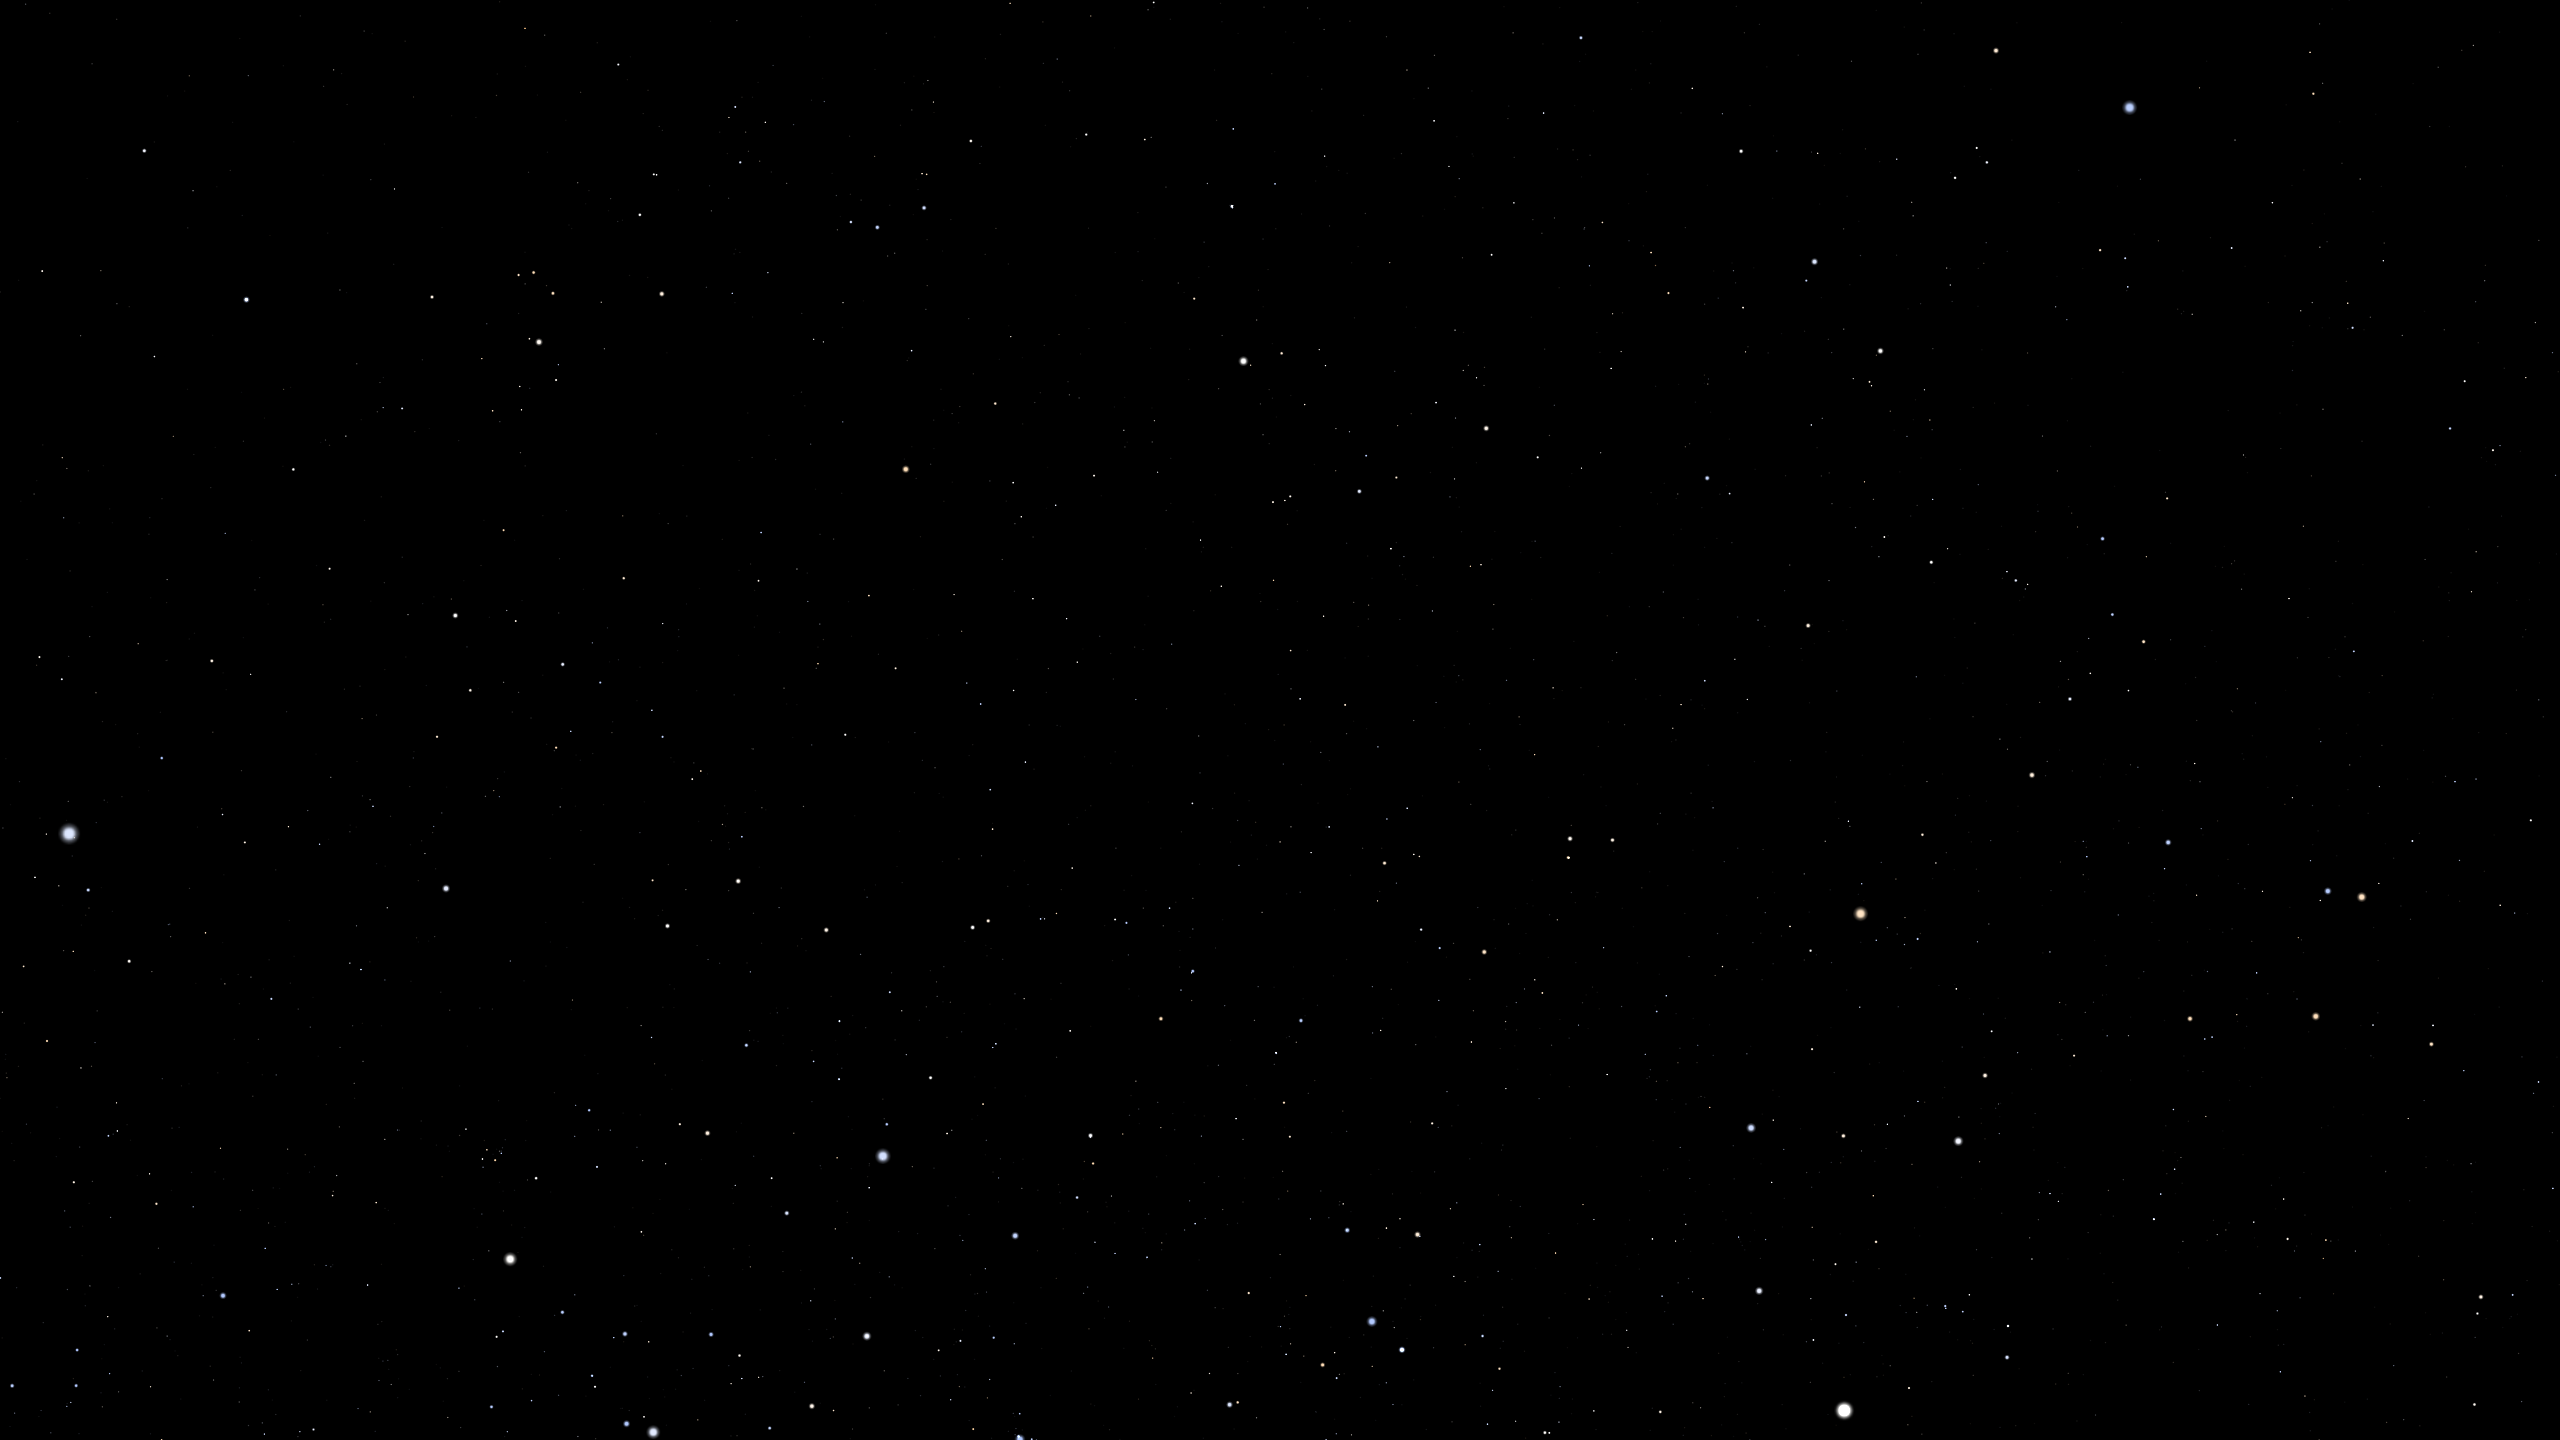
\includegraphics[width=0.9\linewidth]{stars_000}
   \caption{Example image of star field from Stellarium}
   \label{fig:star_img}
\end{figure}

\subsection{Preprocessing}

\begin{figure}[H]
  \centering
   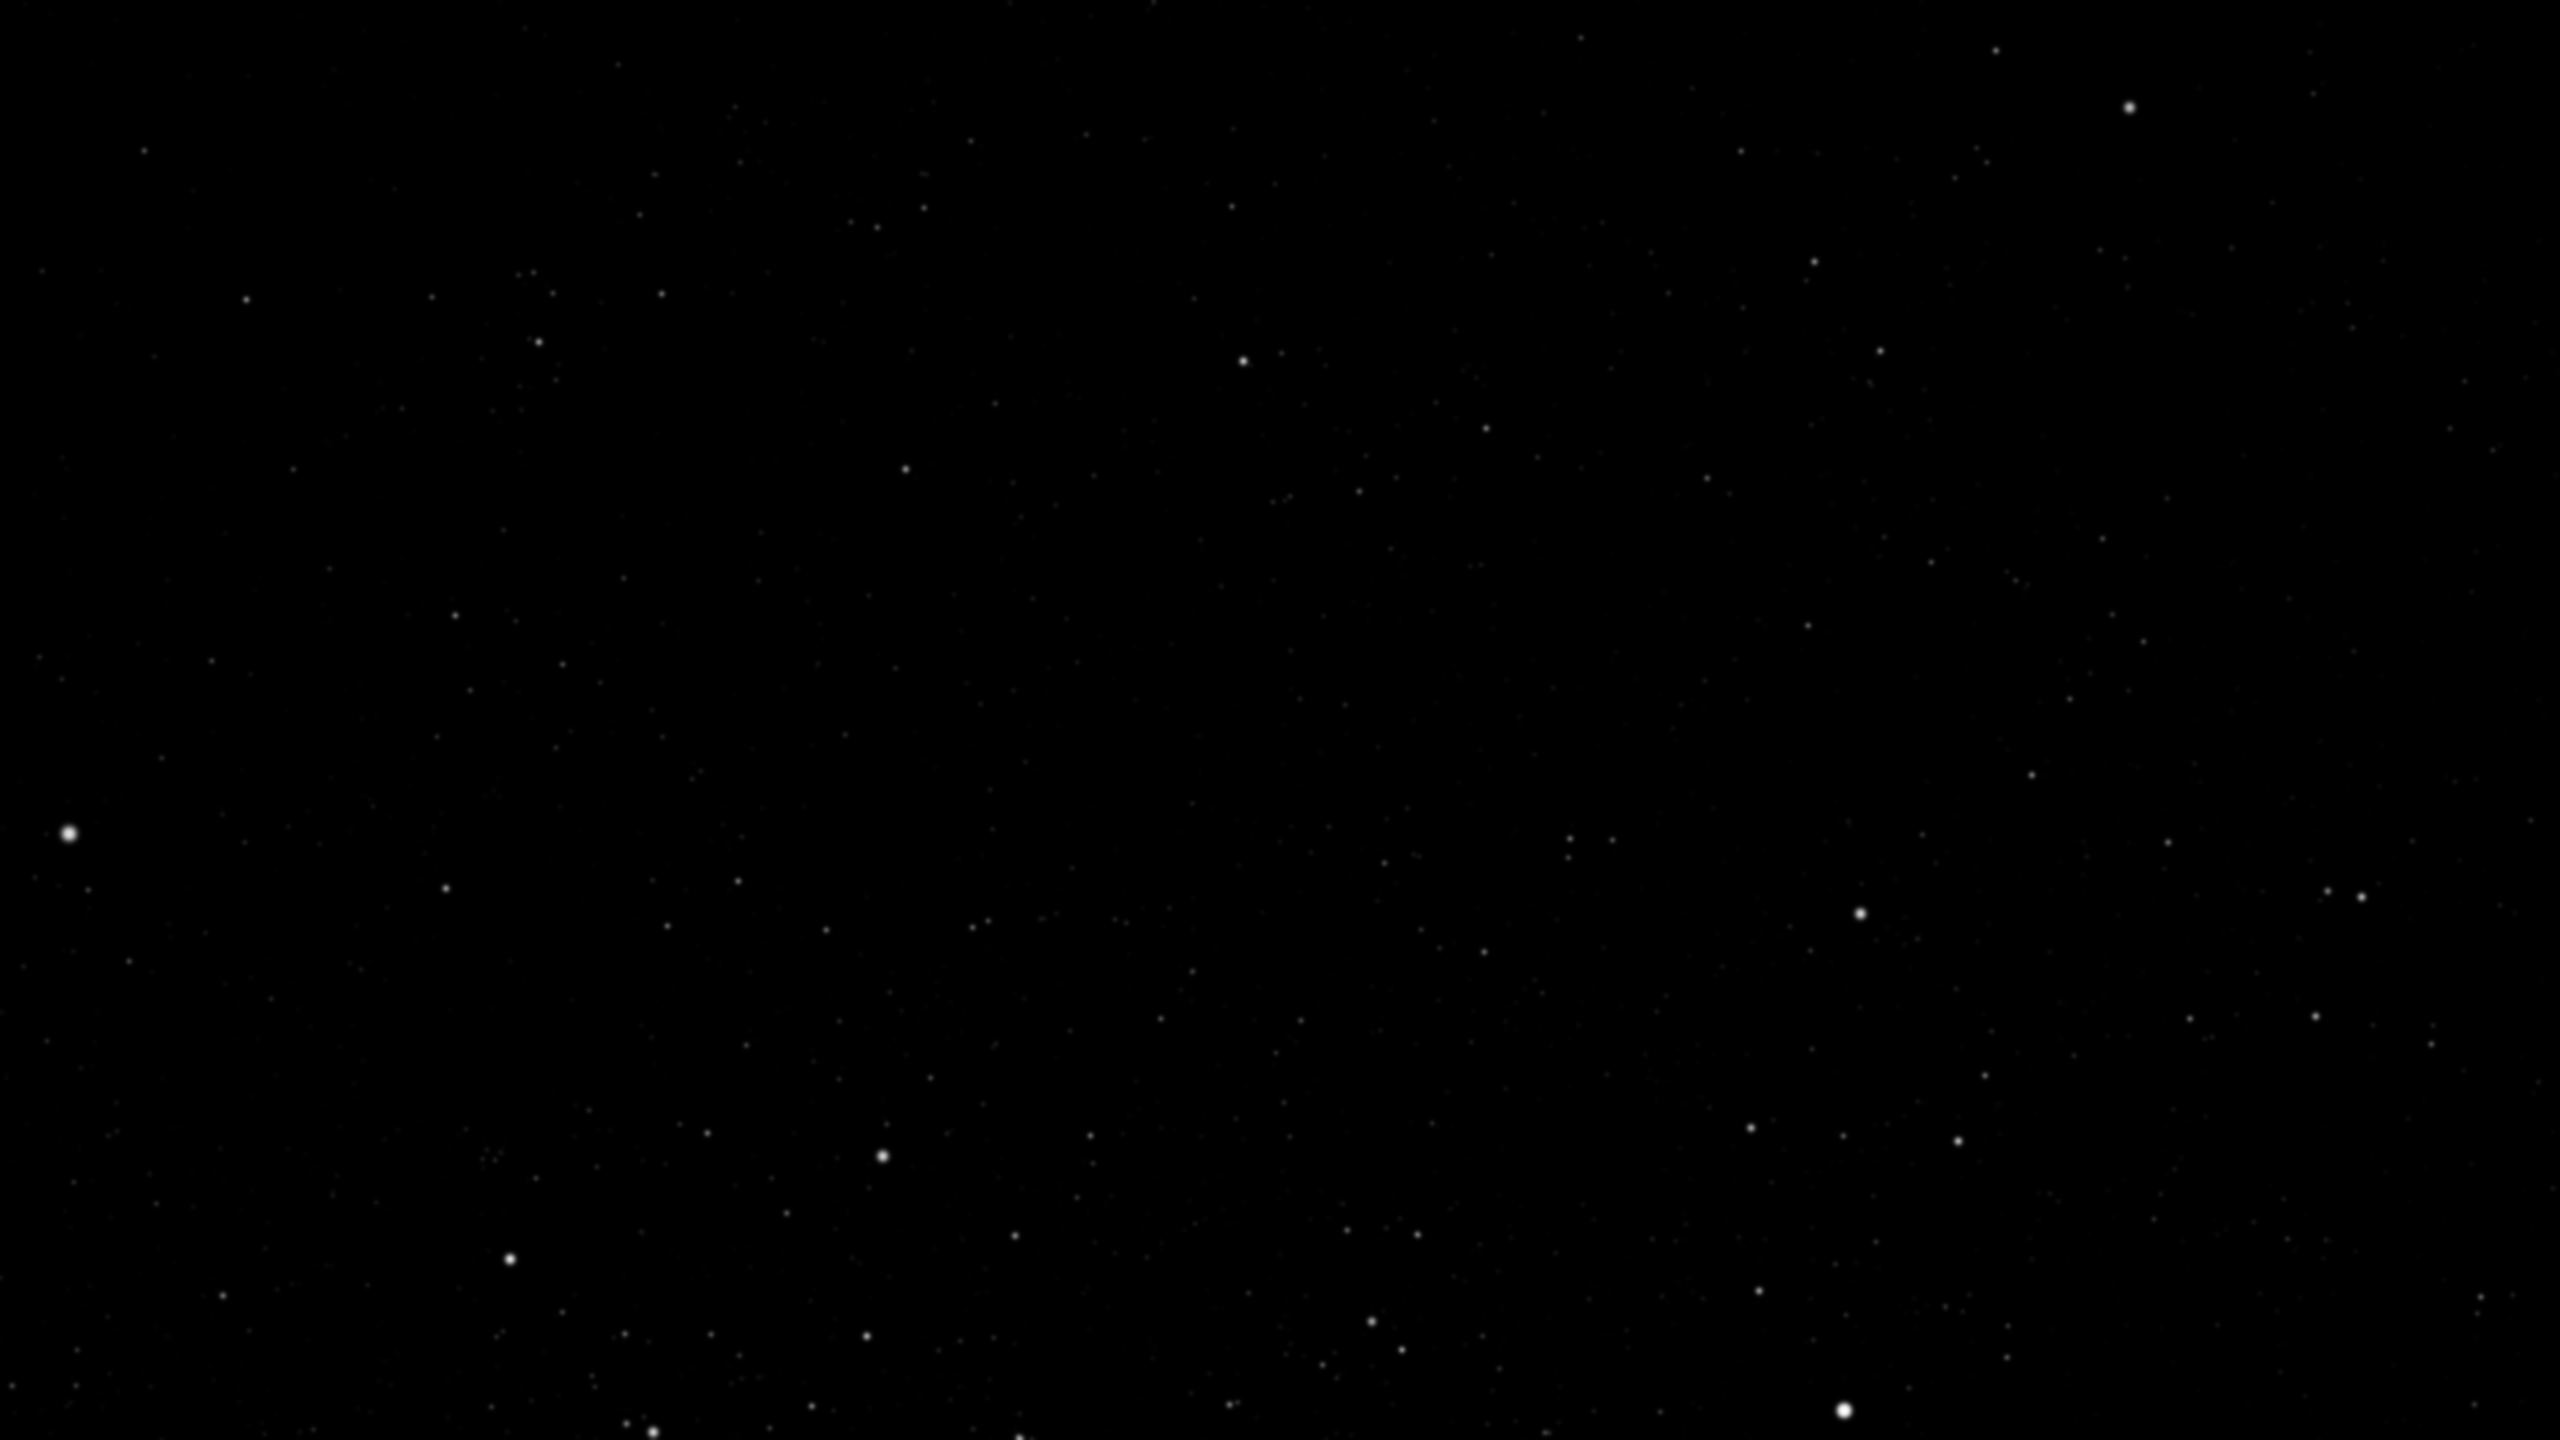
\includegraphics[width=0.9\linewidth]{gauss}
   \caption{Gaussian blur applied to star image}
   \label{fig:star_gauss}
\end{figure}

\begin{figure}[H]
  \centering
   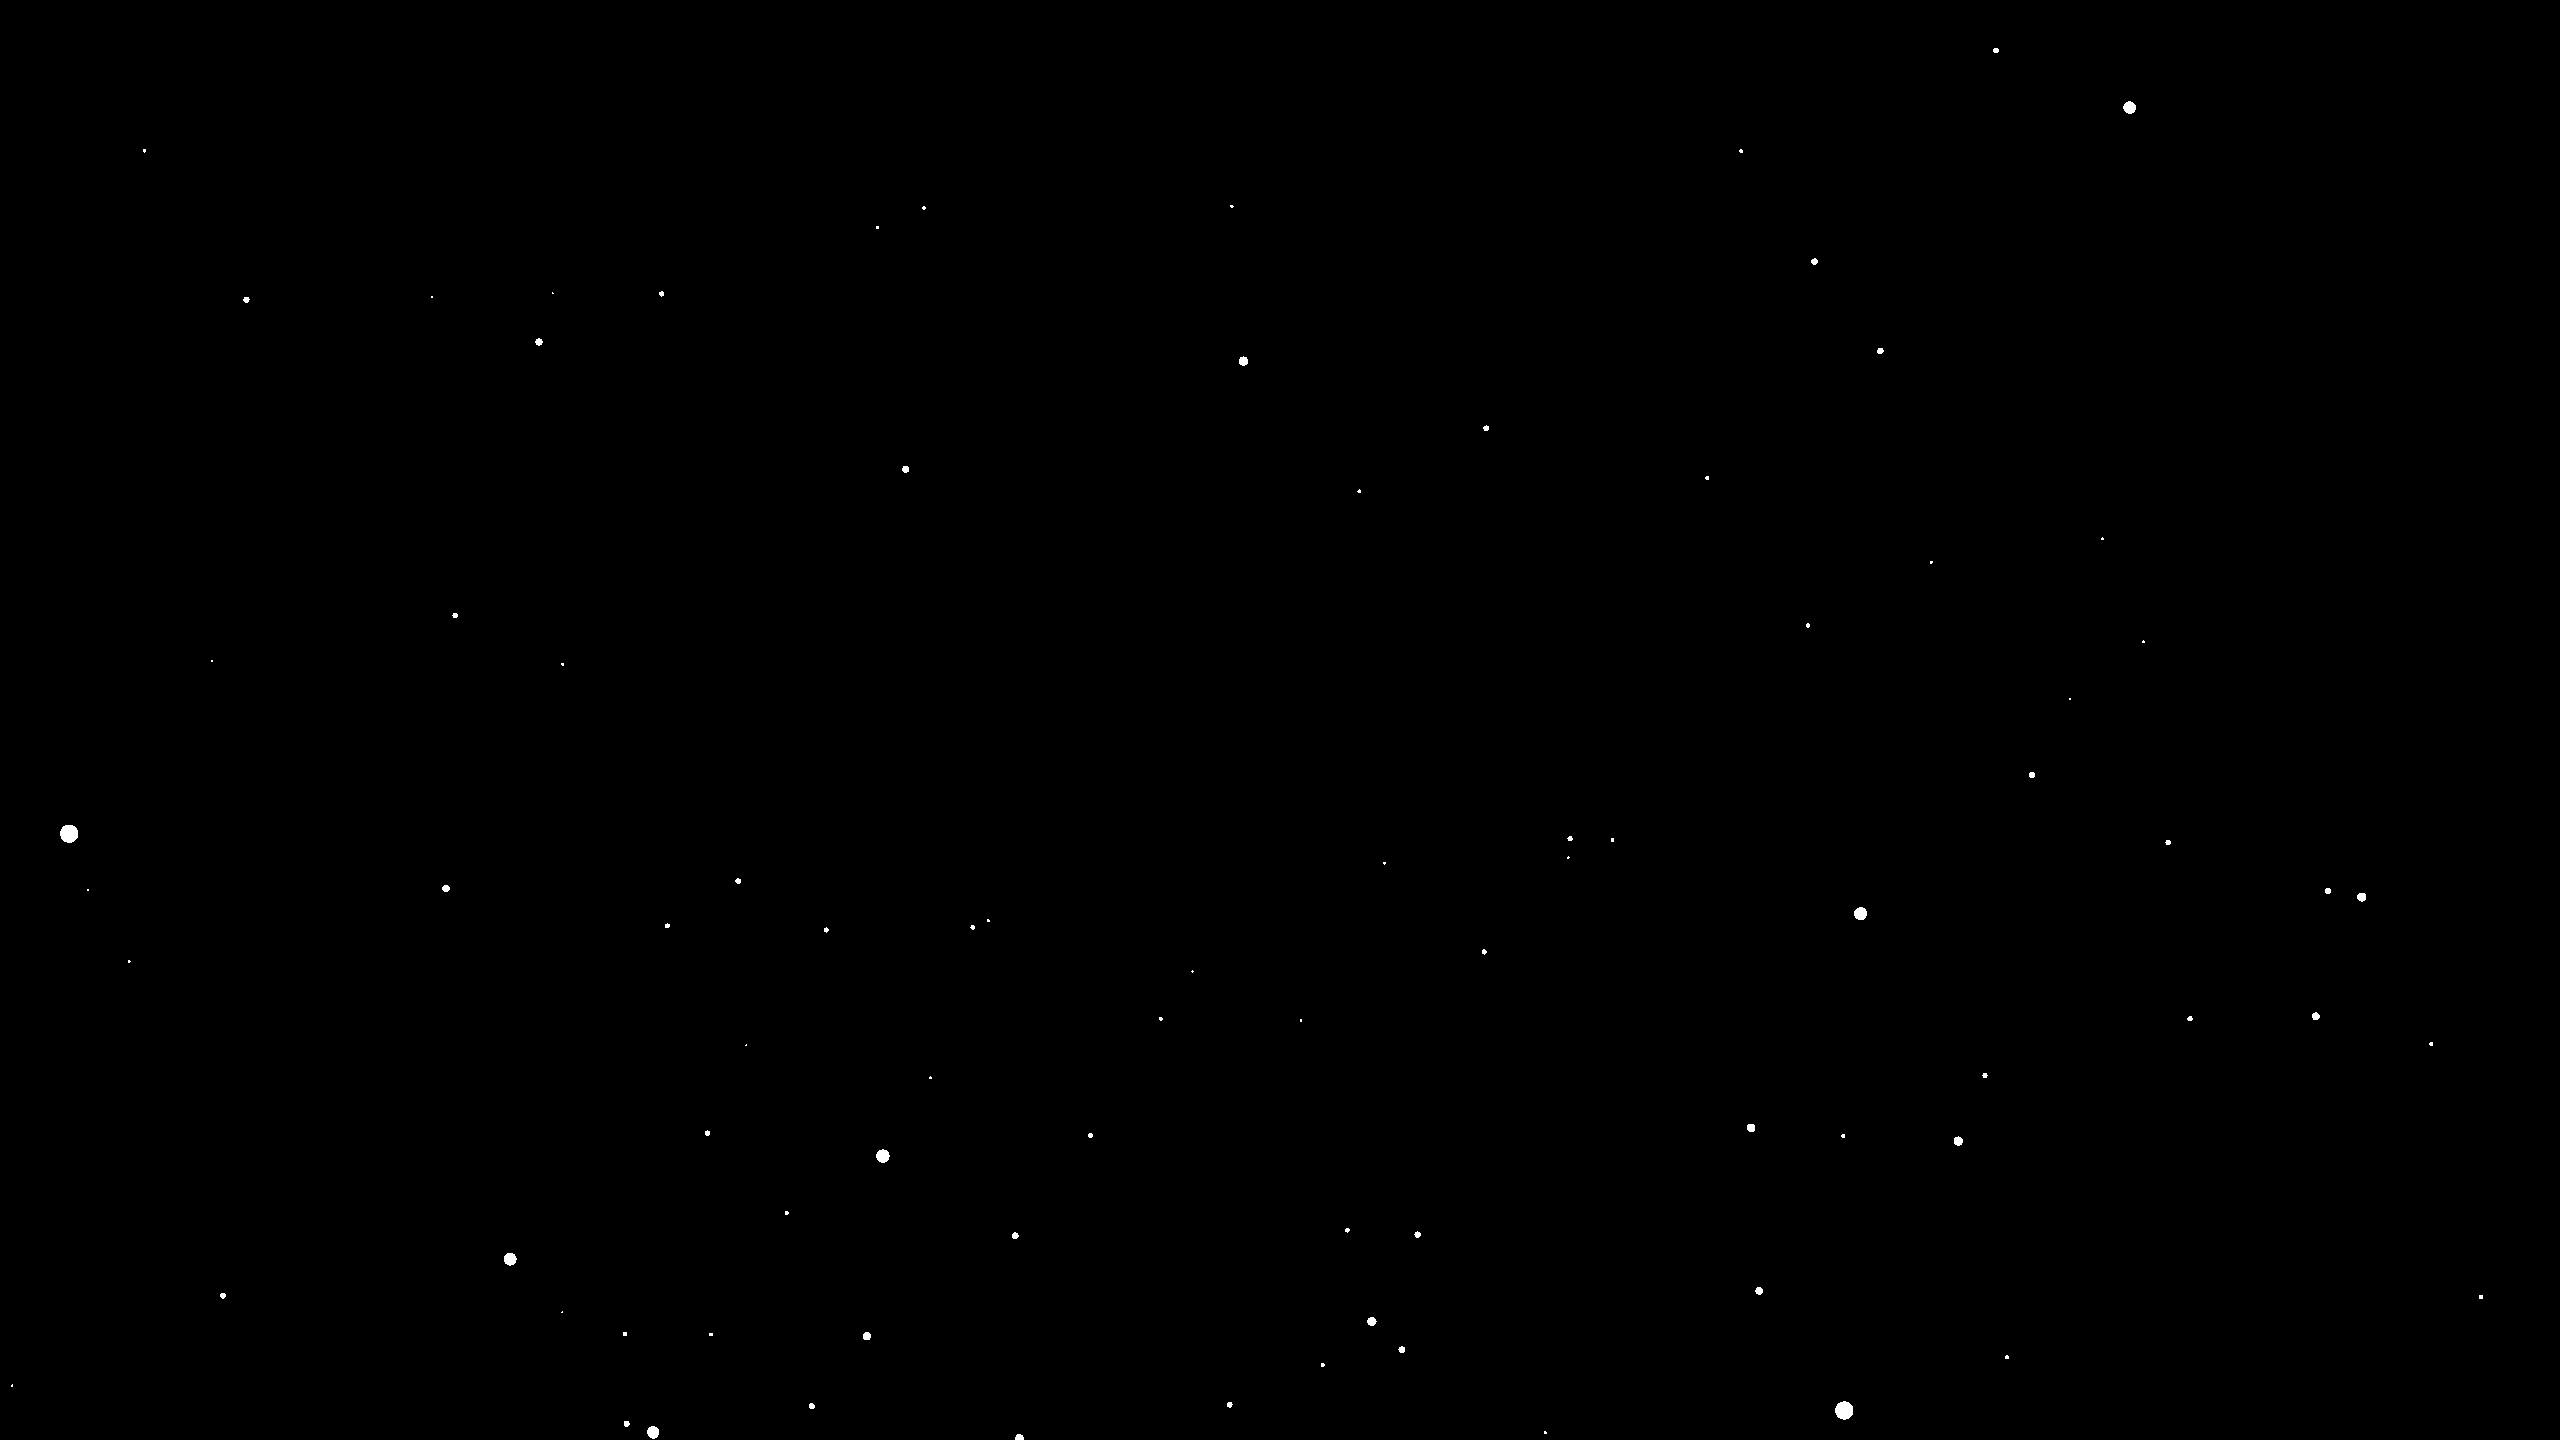
\includegraphics[width=0.9\linewidth]{binary}
   \caption{Result of binarizing the Gaussian blurred image}
   \label{fig:star_binary}
\end{figure}

\subsection{Feature extraction}

\begin{figure}[H]
  \centering
   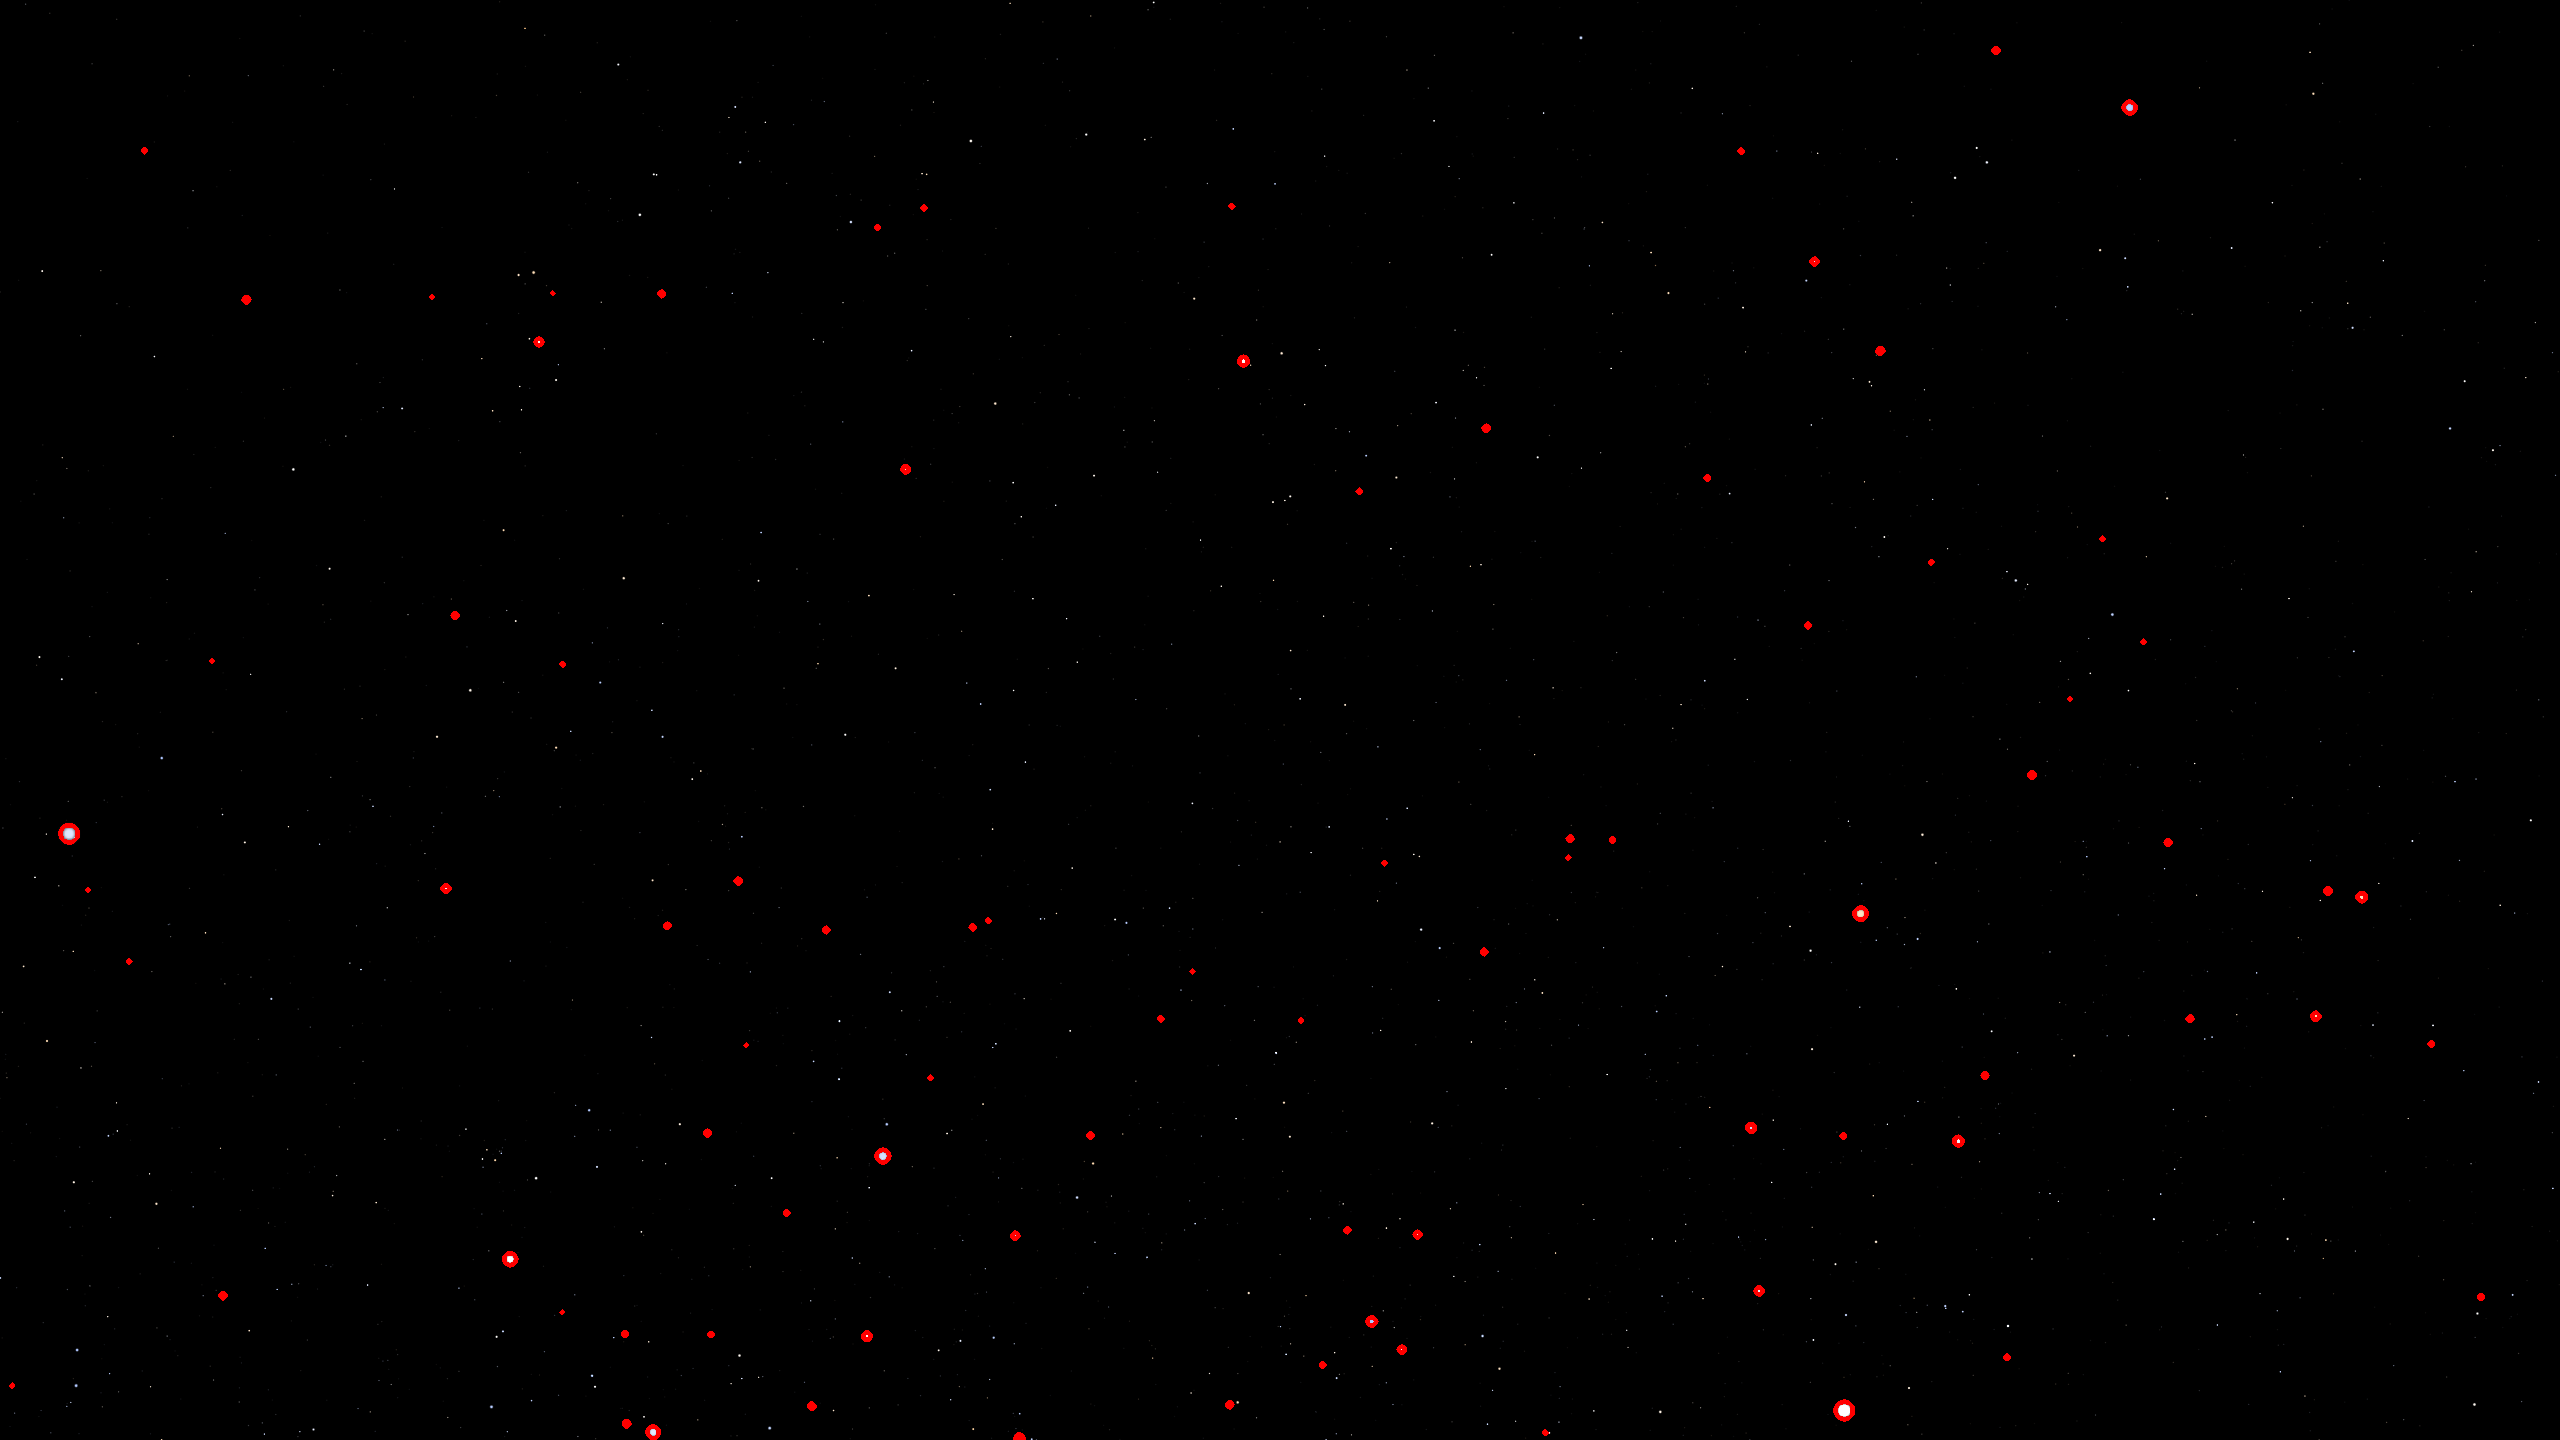
\includegraphics[width=0.9\linewidth]{all_contours}
   \caption{Result of locating global contours}
   \label{fig:star_contours}
\end{figure}

\begin{figure}[H]
  \centering
   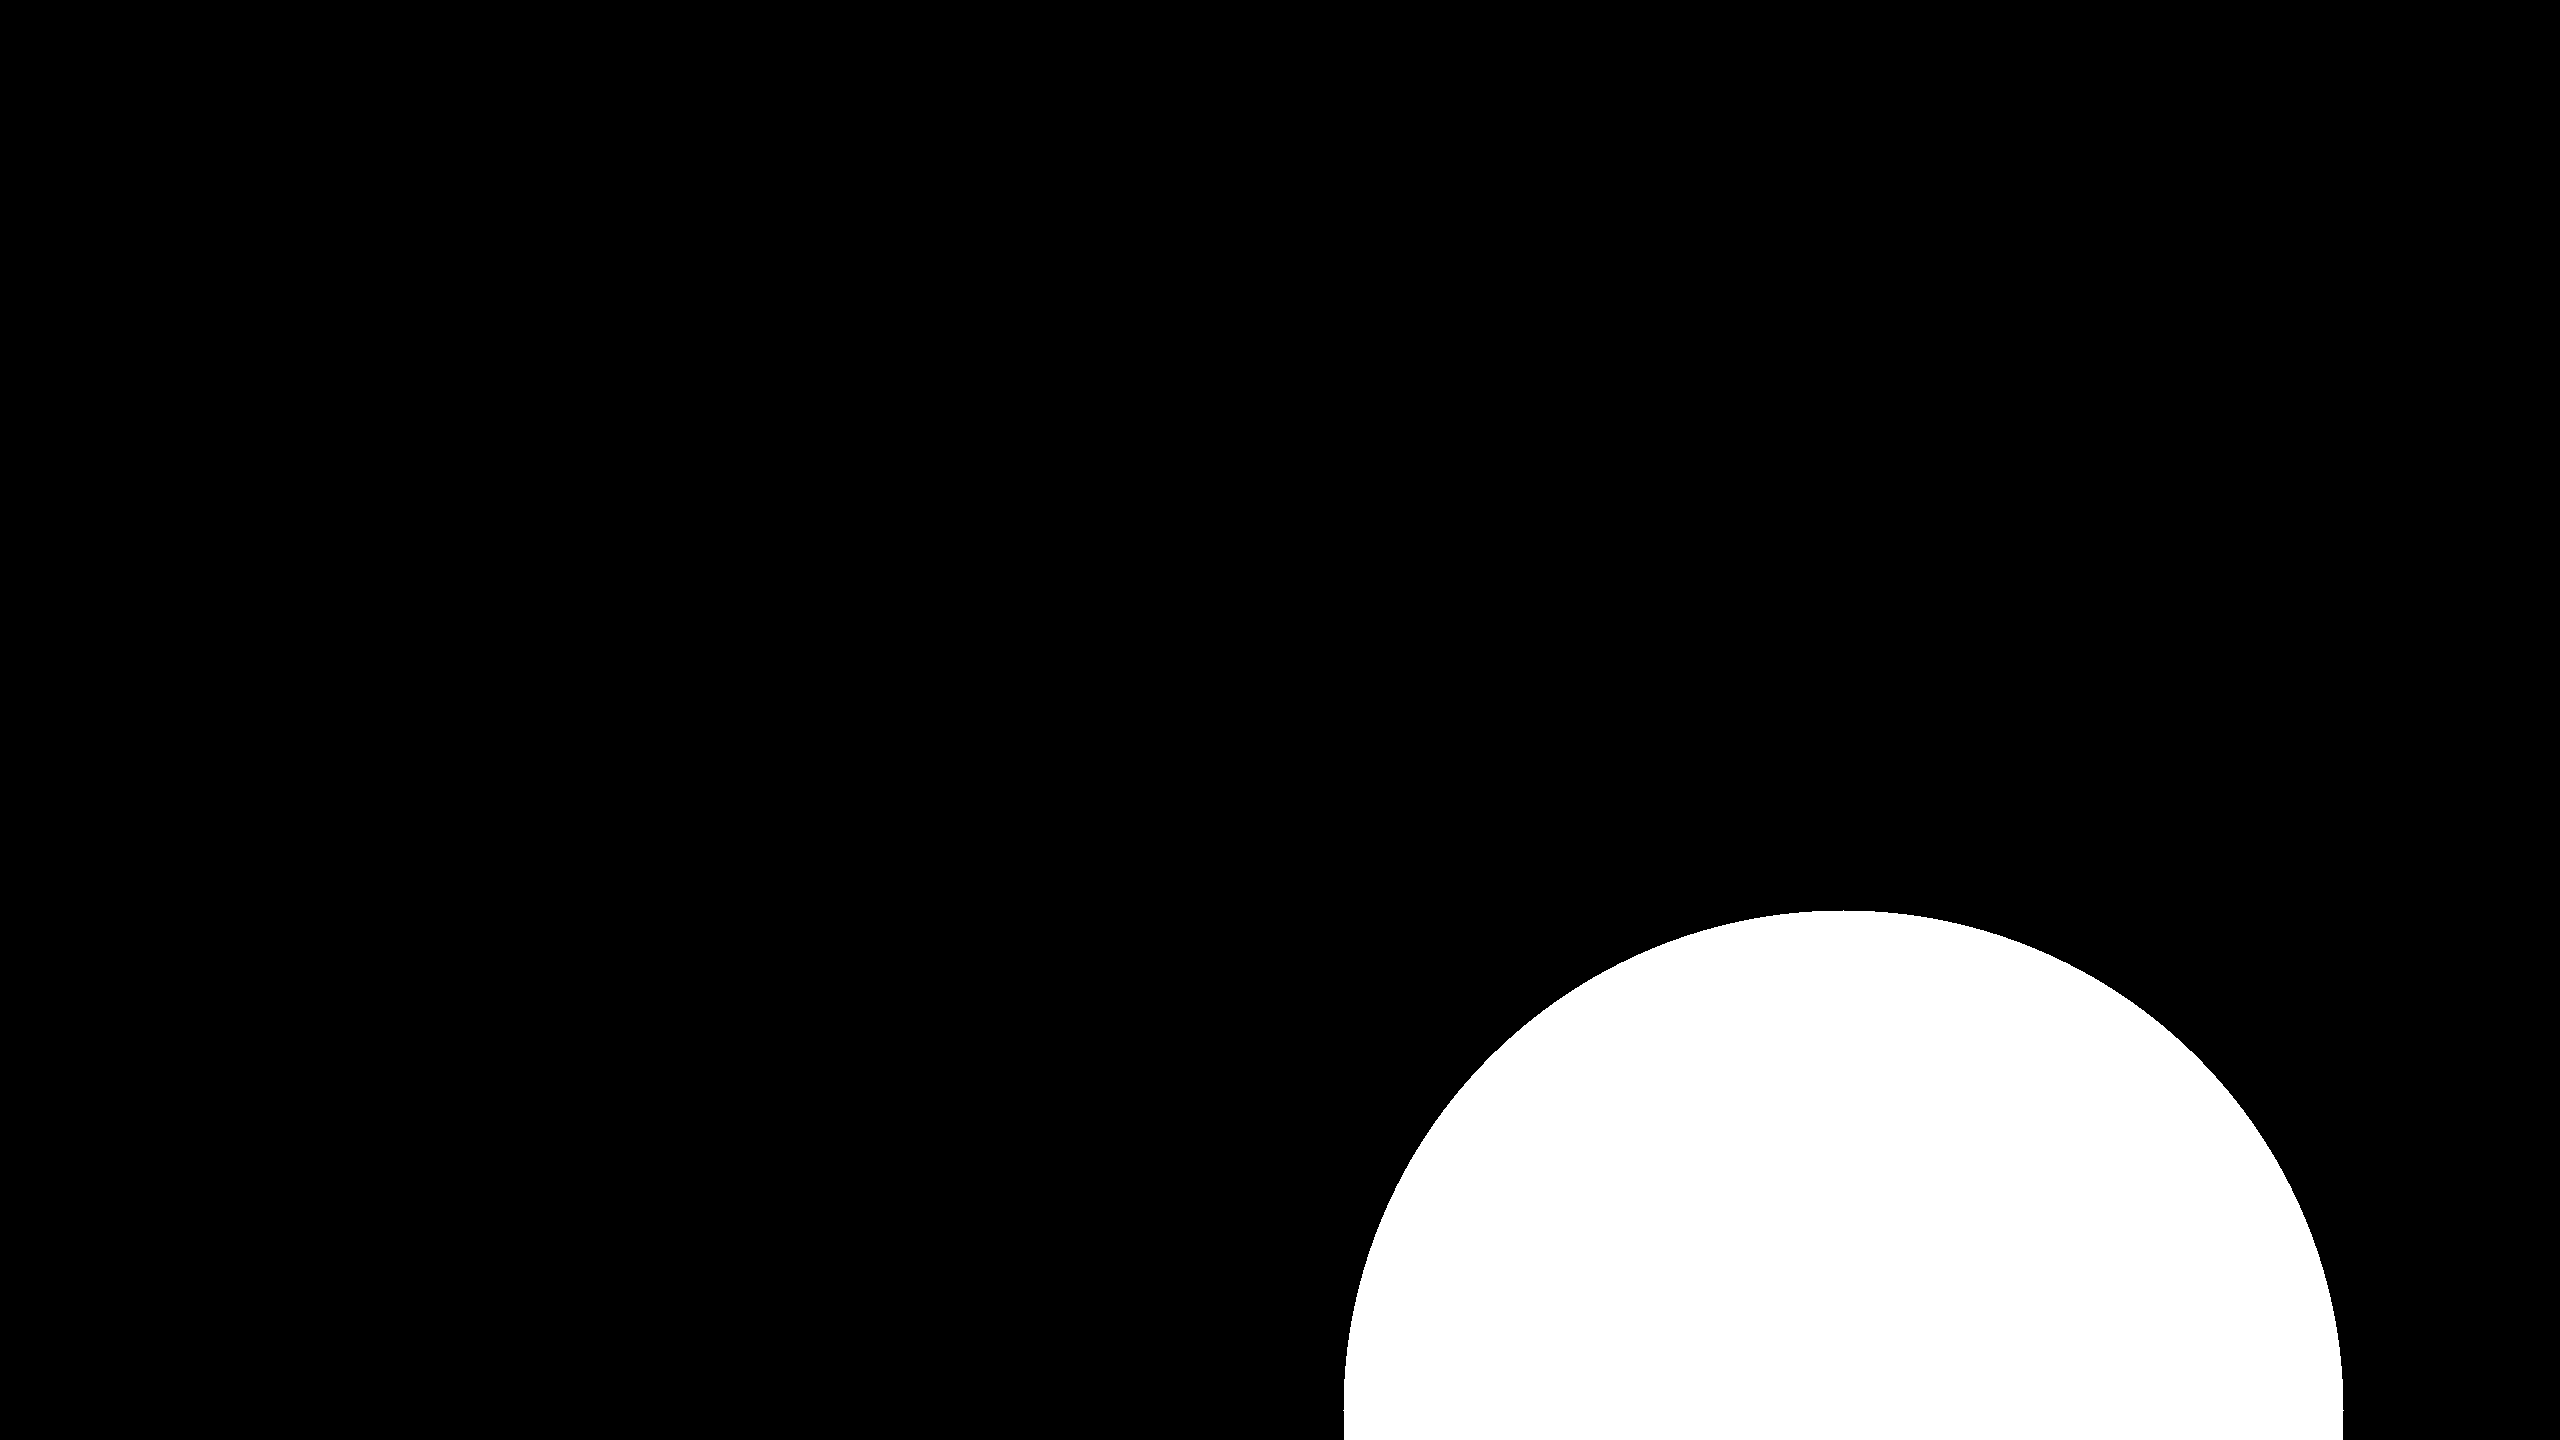
\includegraphics[width=0.9\linewidth]{mask}
   \caption{Circular mask around largest detected contour}
   \label{fig:star_mask}
\end{figure}

\begin{figure}[H]
  \centering
   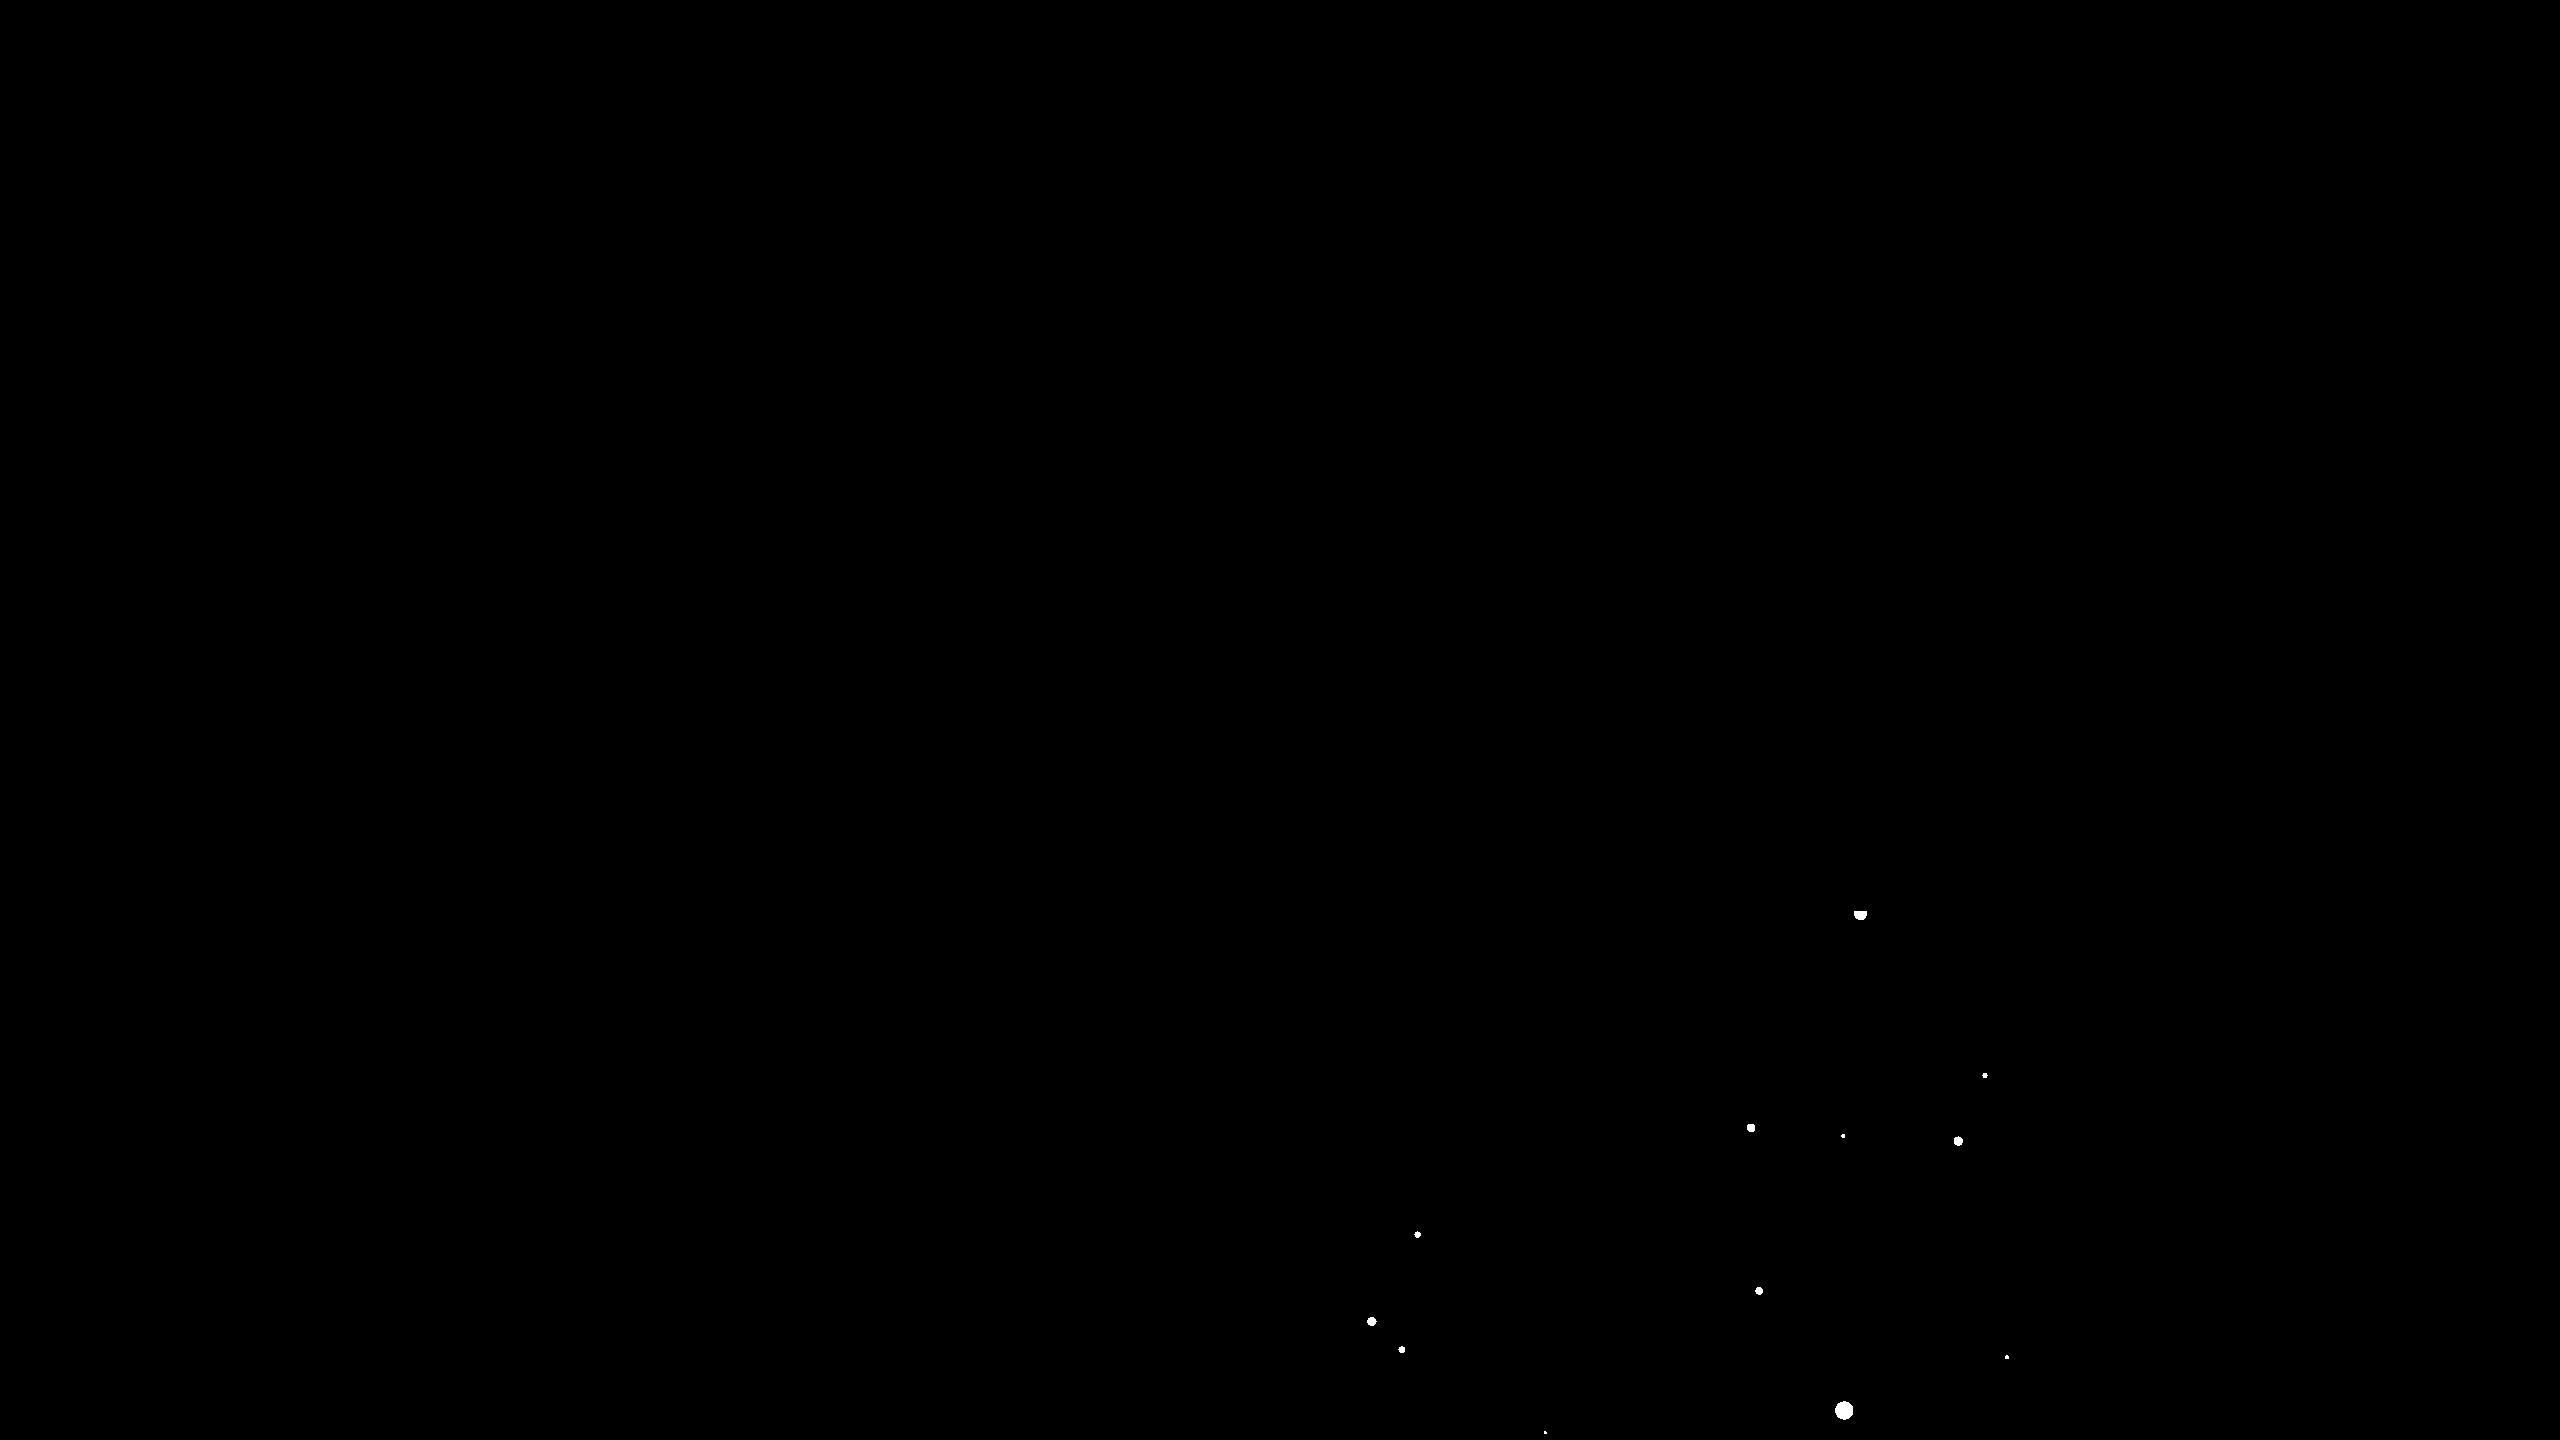
\includegraphics[width=0.9\linewidth]{masked}
   \caption{Result of applying the mask to the binarized image}
   \label{fig:star_masked}
\end{figure}

\begin{figure}[H]
  \centering
   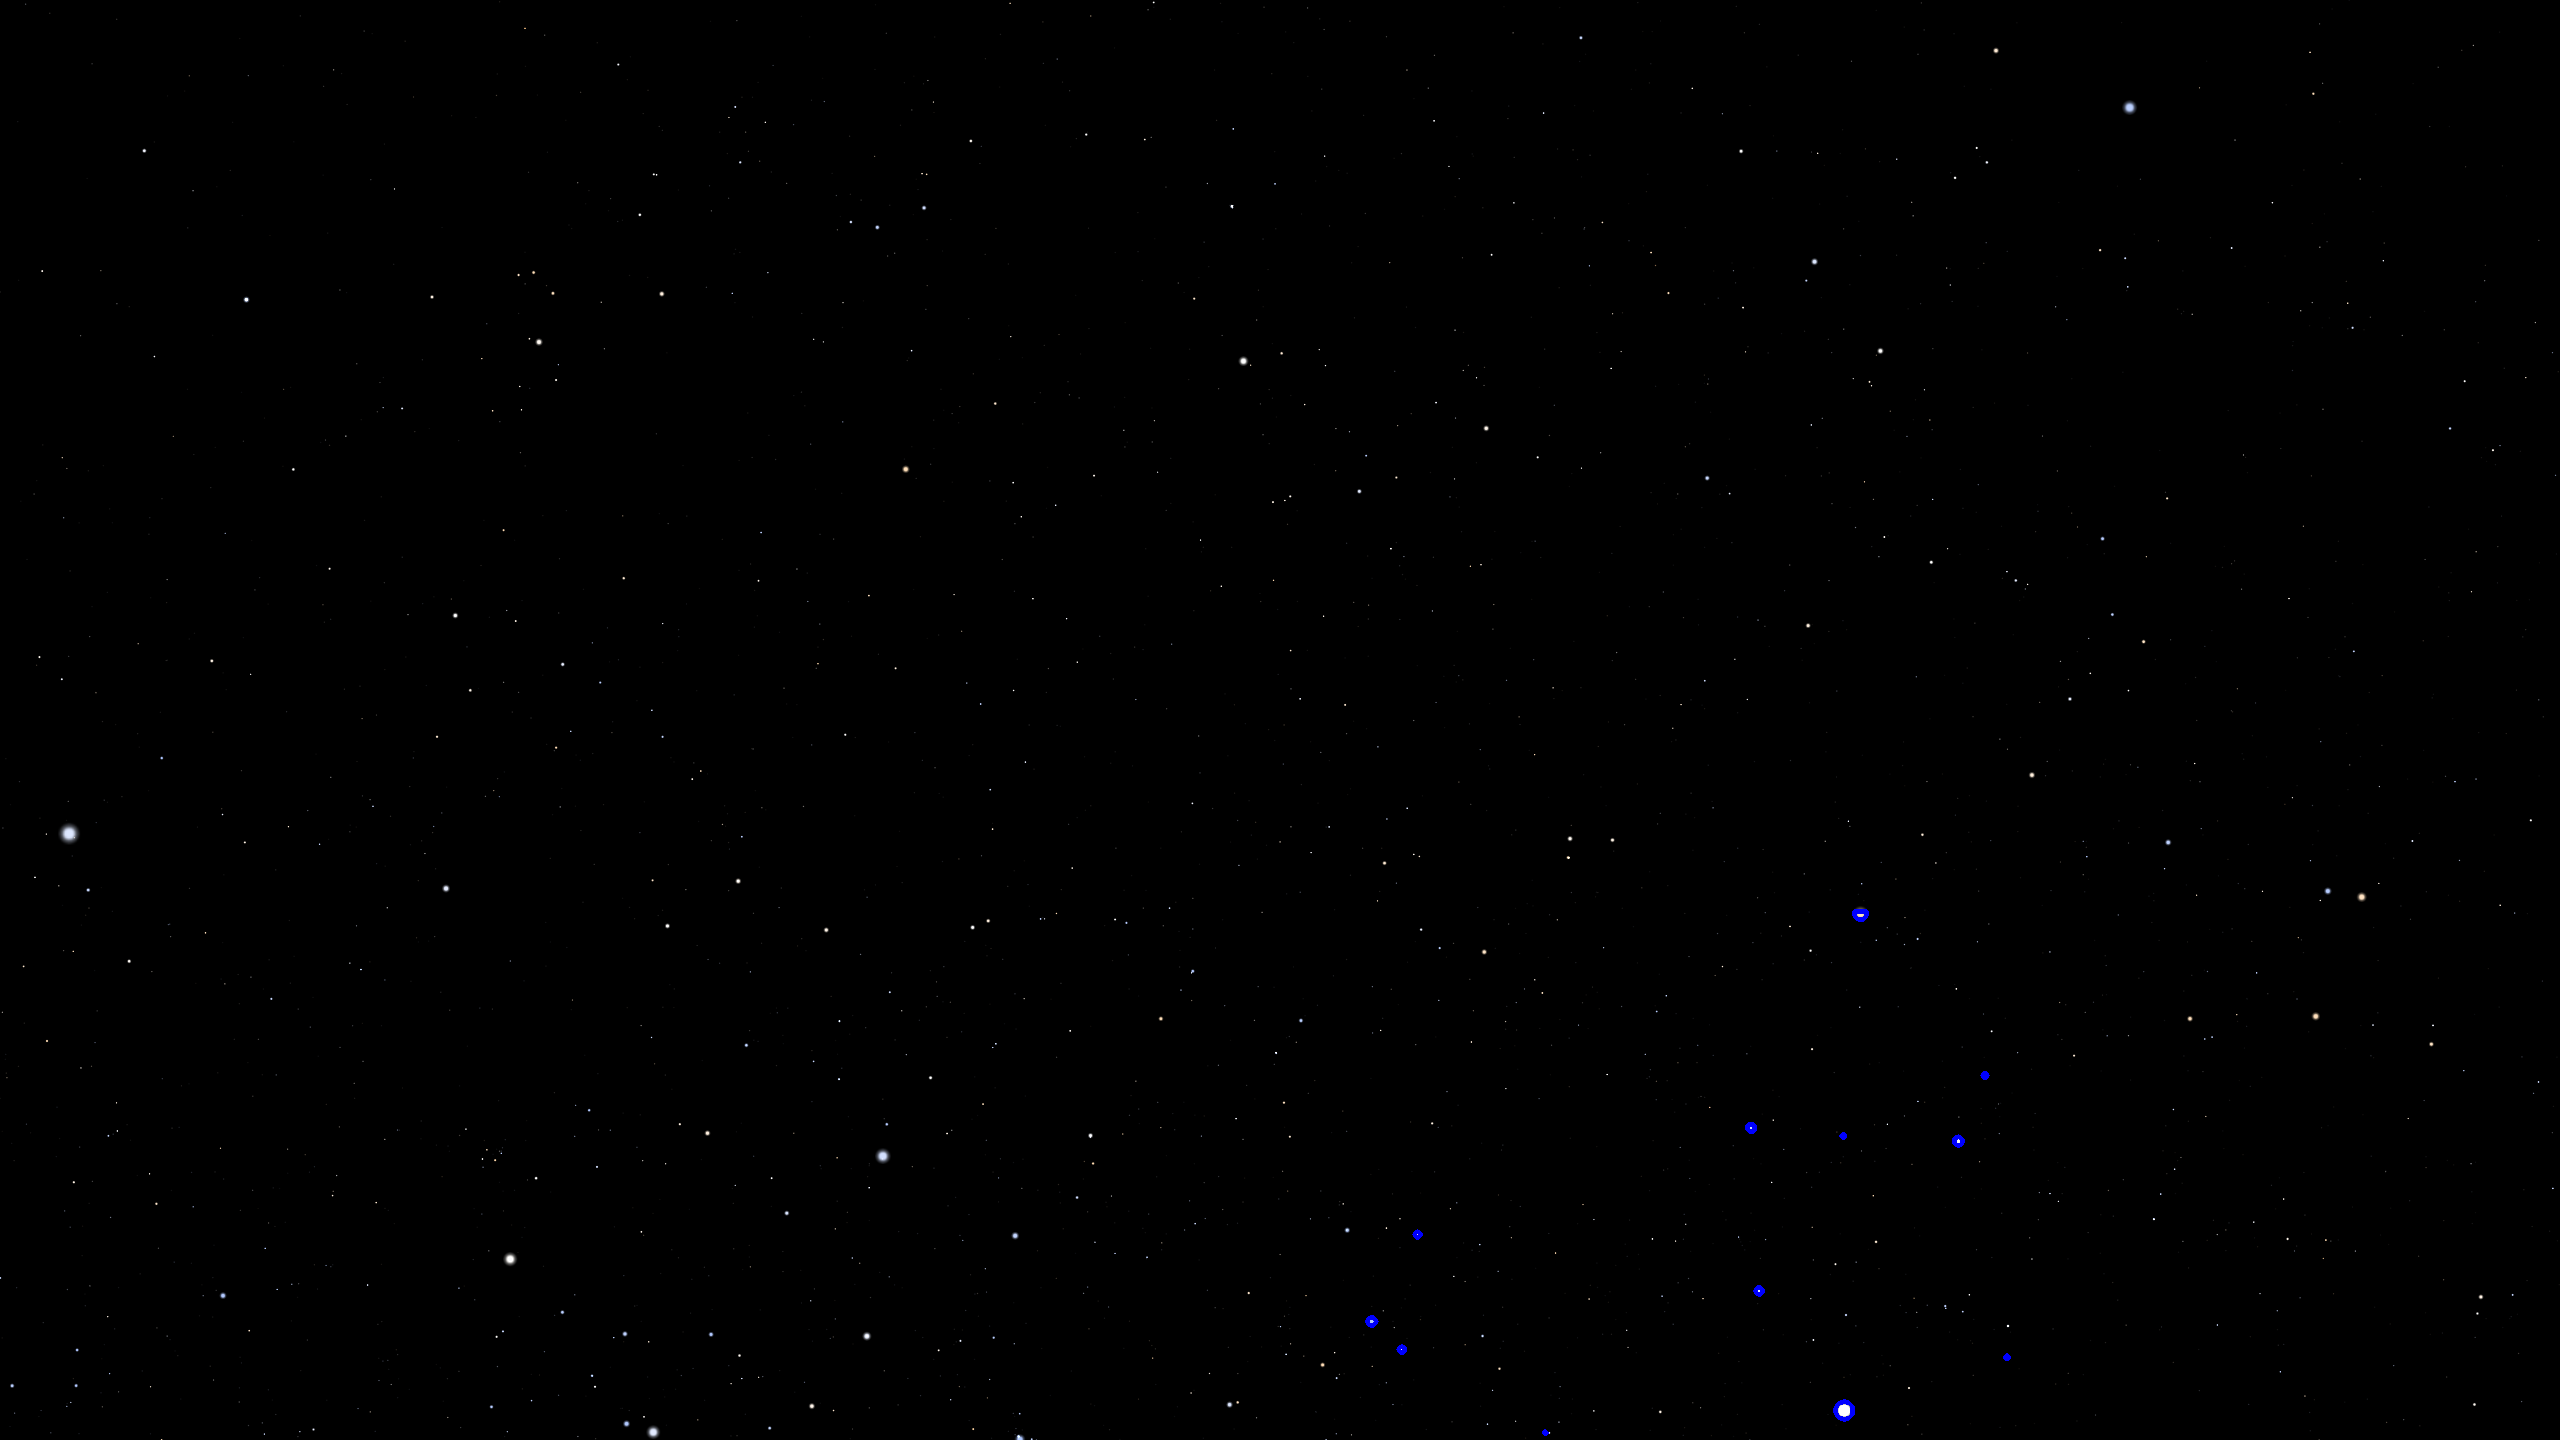
\includegraphics[width=0.9\linewidth]{local_contours}
   \caption{Result of locating contours in the masked region}
   \label{fig:star_local_contours}
\end{figure}

\begin{figure}[H]
  \centering
   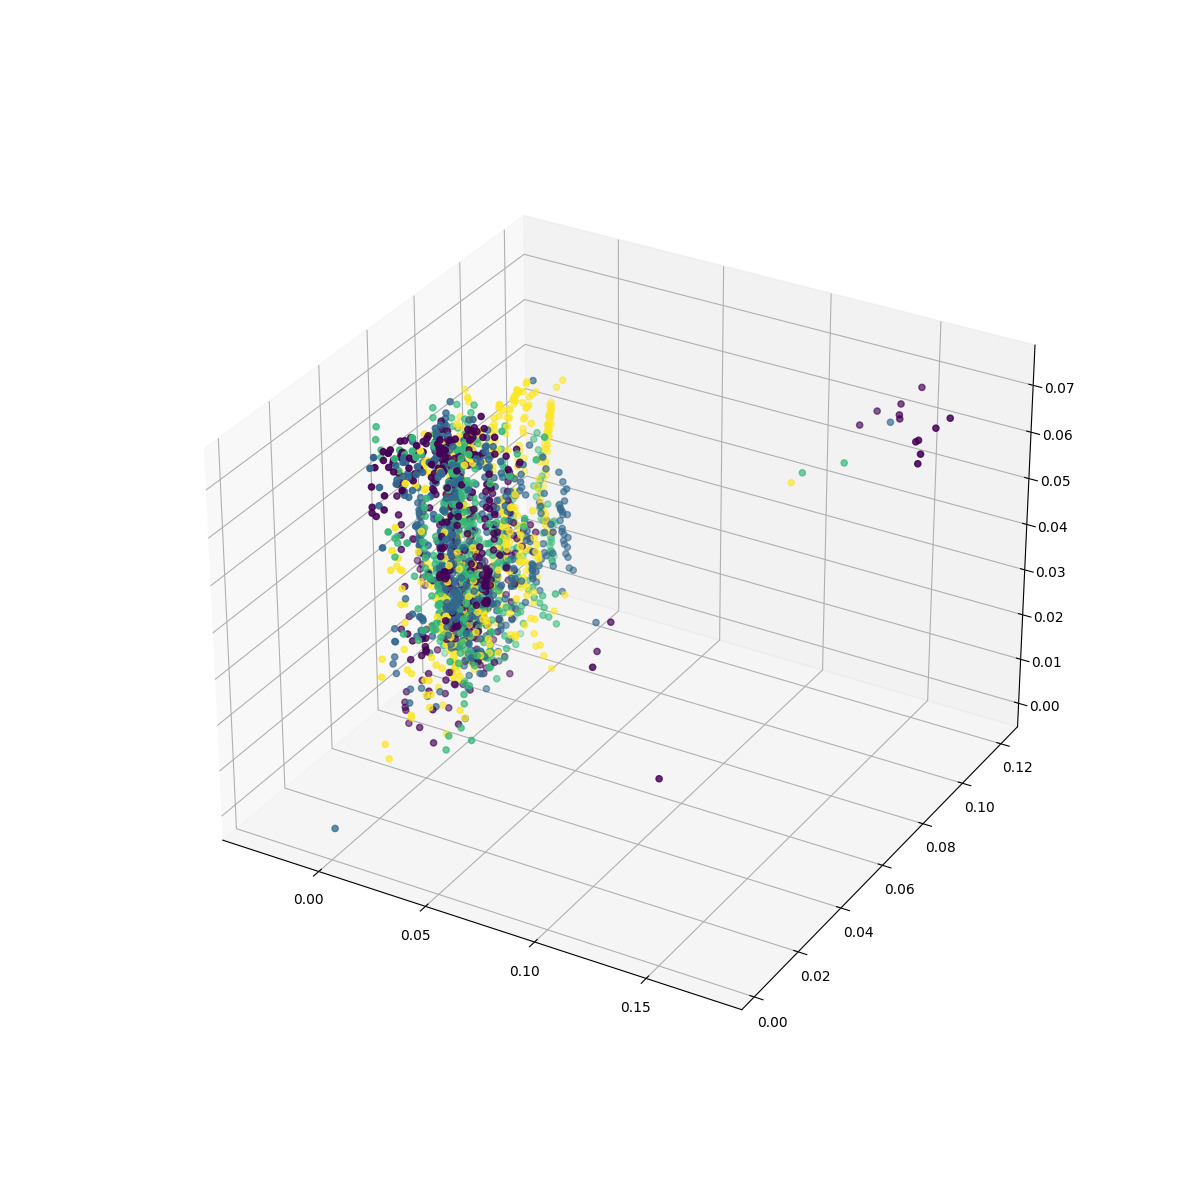
\includegraphics[width=0.9\linewidth, trim={14em, 12em, 9em, 15em}, clip]{pca}
   \caption{\acrshort{pca} applied to the normalized training data}
   \label{fig:pca}
\end{figure}

\section{Alternate Method}
\label{sec:alt_method}

\subsection{\acrlong{cnn}}

\begin{figure}[H]
  \centering
   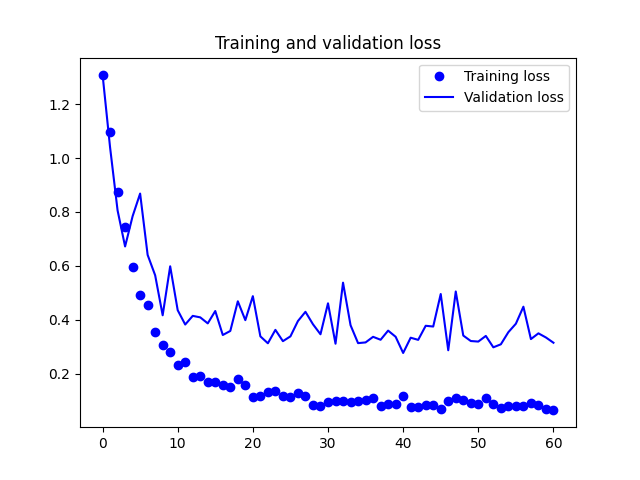
\includegraphics[width=0.9\linewidth, trim={3em, 2em, 4em, 4em}, clip]{cnn_loss}
   \caption{\acrshort{cnn} training and validation loss}
   \label{fig:cnn_loss}
\end{figure}

\begin{figure}[H]
  \centering
   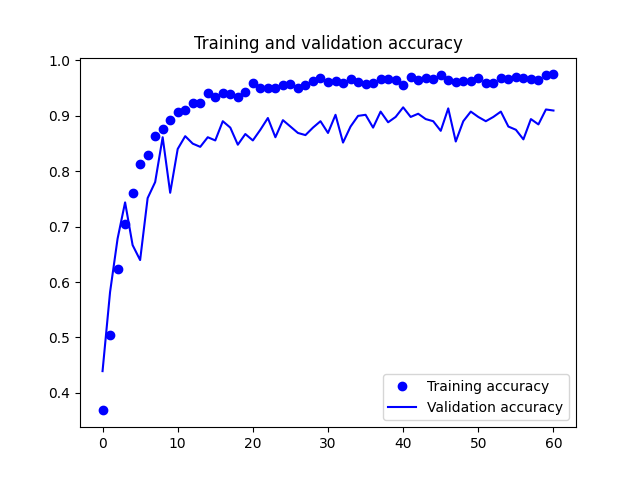
\includegraphics[width=0.9\linewidth, trim={3em, 2em, 4em, 4em}, clip]{cnn_accuracy}
   \caption{\acrshort{cnn} training and validation accuracy}
   \label{fig:cnn_accuracy}
\end{figure}

\subsection{Dataset Augmentation}

\begin{figure}[H]
  \centering
  \begin{subfigure}{.33\linewidth}
    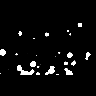
\includegraphics[width=\linewidth]{img_aug}
    \caption{$0^\circ$ rotation}
    \label{fig:img_aug_0}
  \end{subfigure}
  \qquad
  \begin{subfigure}{0.33\linewidth}
    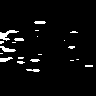
\includegraphics[width=\linewidth]{img_aug_rot_90}
    \caption{$90^\circ$ rotation}
    \label{fig:img_aug_90}
  \end{subfigure}
  
  \begin{subfigure}{0.33\linewidth}
    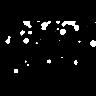
\includegraphics[width=\linewidth]{img_aug_rot_180}
    \caption{$180^\circ$ rotation}
    \label{fig:img_aug_180}
  \end{subfigure}
  \qquad
  \begin{subfigure}{0.33\linewidth}
    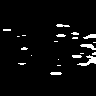
\includegraphics[width=\linewidth]{img_aug_rot_270}
    \caption{$270^\circ$ rotation}
    \label{fig:img_aug_270}
  \end{subfigure}
  \caption{Example of augmented dataset for training the \acrlong{cnn}}
  \label{fig:cnn_aug_imgs}
\end{figure}

\begin{figure}[H]
  \centering
   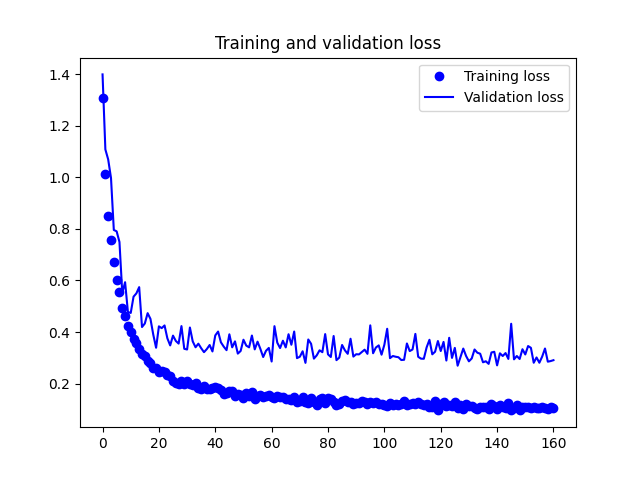
\includegraphics[width=0.9\linewidth, trim={3em, 2em, 4em, 4em}, clip]{cnn_aug_loss}
   \caption{\acrshort{cnn} (augmented dataset) training and validation loss}
   \label{fig:cnn_aug_loss}
\end{figure}

\begin{figure}[H]
  \centering
   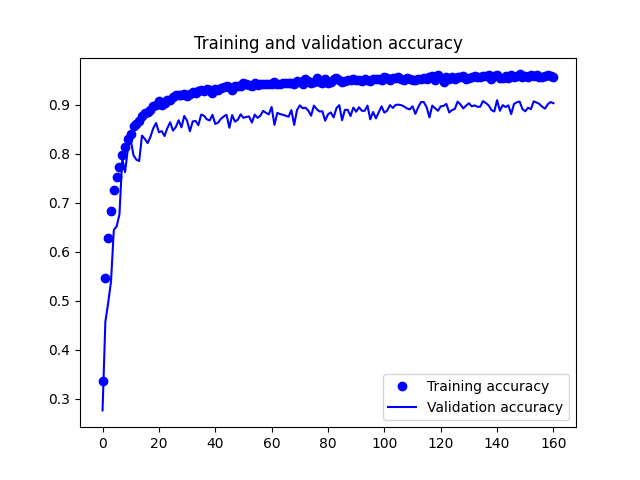
\includegraphics[width=0.9\linewidth, trim={3em, 2em, 4em, 4em}, clip]{cnn_aug_accuracy}
   \caption{\acrshort{cnn} (augmented dataset) training and validation accuracy}
   \label{fig:cnn_aug_accuracy}
\end{figure}

\section{Results}
\label{sec:results}

\begin{table}[H]
  \centering
  \begin{tabular}{*4c}
    \toprule
    Method & \multicolumn{3}{c}{Accuracy} \\
    \midrule
    {} & Training & Validation & Test \\
    \acrshort{svm} & 98.0\% & NA & 88.1\% \\
    \acrshort{cnn} & 98.6\% & 90.9\% & 96.2\% \\
    \acrshort{cnn} (Augmented) & 98.6\% & 90.4\% & 91.1\% \\
    \bottomrule
  \end{tabular}
  \caption{Comparison of classification accuracy for all methods}
  \label{tab:accuracy}
\end{table}

The accuracy for all proposed methods is summarized in Table \ref{tab:accuracy}. From the results, it appears that all 3 supervised models suffer from overfitting as the classification was much more accurate on the training sets than the validation and test sets. The \acrshort{cnn} without augmented data performed the best on the test set with 96.2\% accuracy followed by the same \acrshort{cnn} model trained with the augmented dataset with an accuracy of 91.1\%. The \acrshort{svm} performed the worst of the 3 models with an accuracy of 88.1\% on the test set.

The primary source of error in the \acrshort{svm} algorithm is due to the fact that the features are not exactly unique to the class around the class boundaries. This is due to the fact that the algorithm uses the brightest star and distances to the nearest stars around the brightest star. For example, the brightest star could be present in one image labelled as the North-East sky, but also be visible as the brightest star in an image labelled as the North-West sky. This error is specifically noticeable around the South-East/West sky boundary, which can be observed from the high amount of misclassified stars in the training and test data confusion matrices shown in Figure \ref{fig:svm_res}.

A similar result is observed for the \acrshort{cnn} trained with the augmented data set in that there is a large number of misclassified stars between the South-East/West skies. From this observation, it seems that the \acrshort{cnn} trained on the augmented dataset has created a model which is similar to the \acrshort{svm} trained with the features described in Section \ref{sec:method}. Intuitively, this observation makes sense because the dataset was augmented by rotating the images around the center pixel, which has the impact of making the model more robust with respect to axial rotation. Similarly, the features chosen to train the \acrshort{svm} were chosen such that they would be the same feature values regardless of rotation around the axis. For example, the distance of the brightest star to other stars does not change as the field of view is rotated around the center pixel.

Although the \acrshort{cnn} trained on the original dataset shows the highest accuracy, it is likely that in practice this model would not perform the best because it will not be robust to axial rotation. This robustness is crucial to the satellite as it is unlikely that the satellite will be rotated in such a way that it always aligns with the axially rotation of the images in the supervisory dataset. For this reason, the \acrshort{cnn} trained with the augmented dataset of rotated images is the better candidate for usage in practice.

\begin{figure*}
  \centering
  \begin{subfigure}{.33\linewidth}
    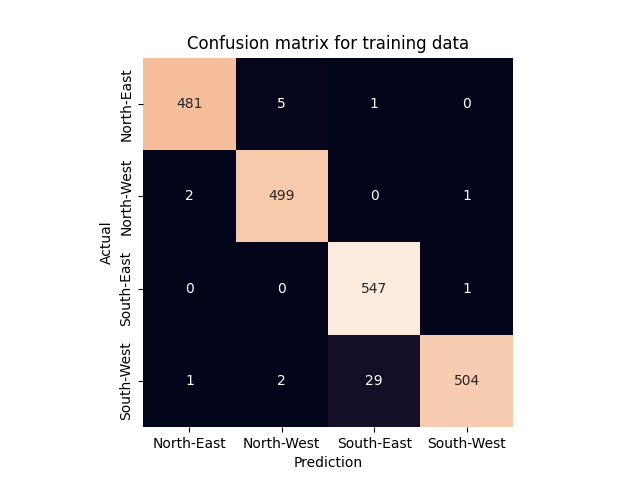
\includegraphics[width=\linewidth, trim={7em, 0em, 9em, 5em}, clip]{svm_cfsn_train}
    \caption{Training data confusion matrix}
    \label{fig:svm_train}
  \end{subfigure}
  \begin{subfigure}{0.33\linewidth}
    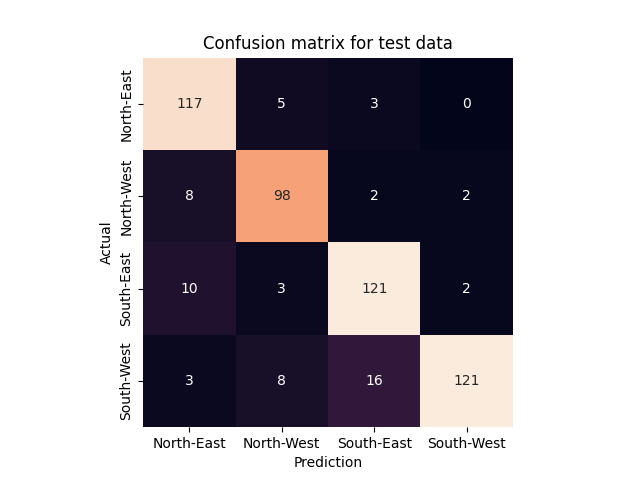
\includegraphics[width=\linewidth, trim={7em, 0em, 9em, 5em}, clip]{svm_cfsn_test}
    \caption{Test data confusion matrix}
    \label{fig:svm_test}
  \end{subfigure}
  \caption{\acrlong{svm} classification results}
  \label{fig:svm_res}
\end{figure*}

\begin{figure*}
  \centering
  \begin{subfigure}{.33\linewidth}
    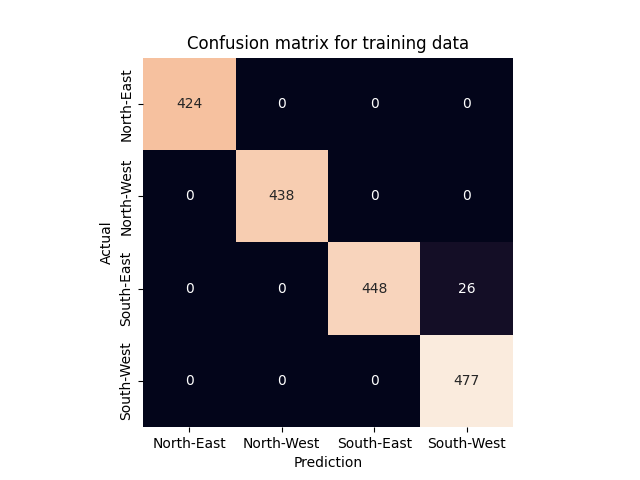
\includegraphics[width=\linewidth, trim={7em, 0em, 9em, 5em}, clip]{cnn_cfsn_train}
    \caption{Training data confusion matrix}
    \label{fig:cnn_train}
  \end{subfigure}
  \begin{subfigure}{0.33\linewidth}
    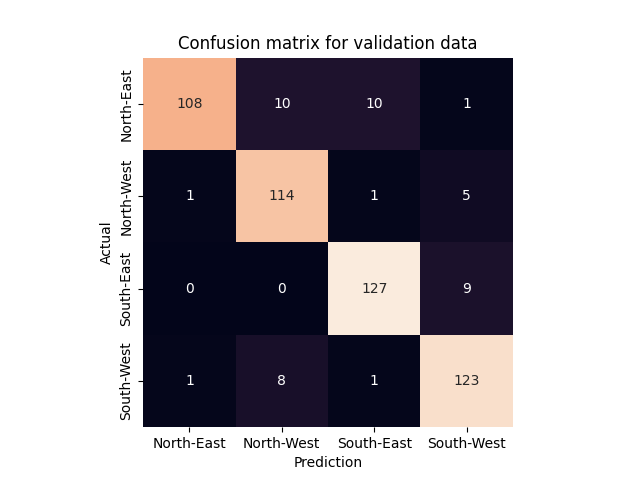
\includegraphics[width=\linewidth, trim={7em, 0em, 9em, 5em}, clip]{cnn_cfsn_valid}
    \caption{Validation data confusion matrix}
    \label{fig:cnn_valid}
  \end{subfigure}
  \begin{subfigure}{0.33\linewidth}
    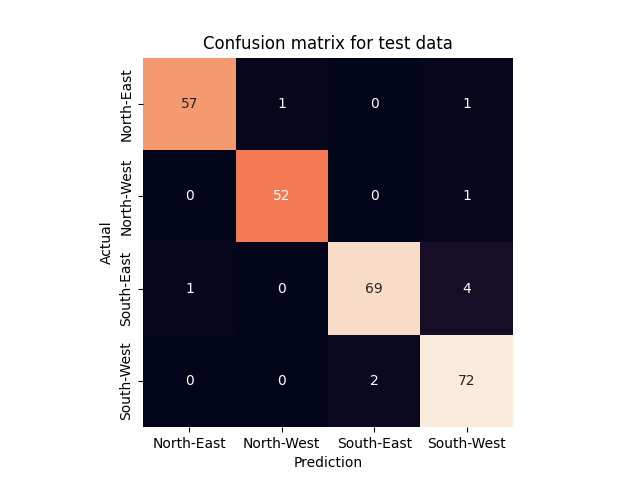
\includegraphics[width=\linewidth, trim={7em, 0em, 9em, 5em}, clip]{cnn_cfsn_test}
    \caption{Test data confusion matrix}
    \label{fig:cnn_test}
  \end{subfigure}
  \caption{\acrshort{cnn} classification results}
  \label{fig:cnn_res}
\end{figure*}

\begin{figure*}
  \centering
  \begin{subfigure}{.33\linewidth}
    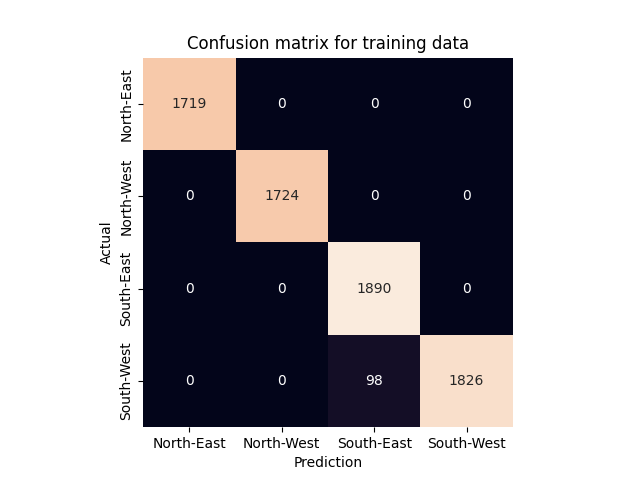
\includegraphics[width=\linewidth, trim={7em, 0em, 9em, 5em}, clip]{cnn_aug_cfsn_train}
    \caption{Training data confusion matrix}
    \label{fig:cnn_train}
  \end{subfigure}
  \begin{subfigure}{0.33\linewidth}
    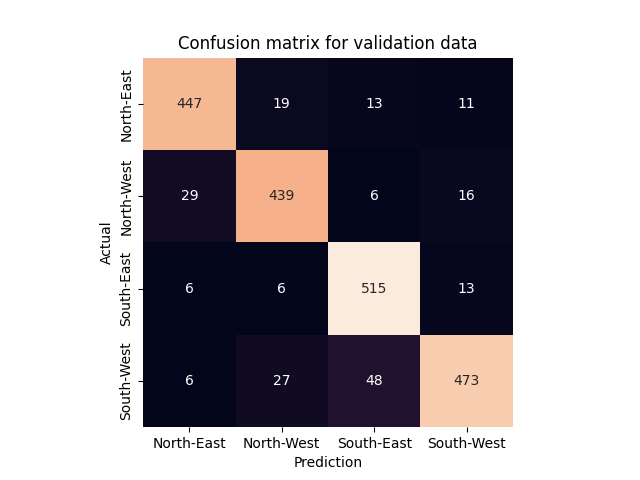
\includegraphics[width=\linewidth, trim={7em, 0em, 9em, 5em}, clip]{cnn_aug_cfsn_valid}
    \caption{Validation data confusion matrix}
    \label{fig:cnn_valid}
  \end{subfigure}
  \begin{subfigure}{0.33\linewidth}
    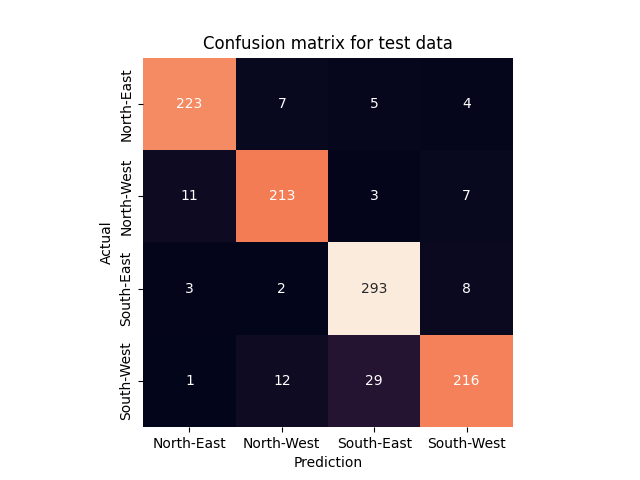
\includegraphics[width=\linewidth, trim={7em, 0em, 9em, 5em}, clip]{cnn_aug_cfsn_test}
    \caption{Test data confusion matrix}
    \label{fig:cnn_test}
  \end{subfigure}
  \caption{\acrshort{cnn} (augmented dataset) classification results}
  \label{fig:cnn_aug_res}
\end{figure*}


\section{Conclusion}
\label{sec:conclusion}

In this paper, a method was proposed to perform satellite attitude determination without an on-board star database. Two approaches were evaluated, both of which relying on usage of supervised learning against a dataset of simulated star field images. The first approach utilized manual feature extraction and classification with an \acrshort{svm}, and the second used a \acrshort{cnn}. The results showed that the \acrshort{cnn} model performed with the highest accuracy on the test set; however, it was determined that the \acrshort{cnn} trained on the augmented dataset would be more useful in practice due to the robustness to axial rotation.

The results indicate that the proposed methods are not sufficient to perform highly accurate attitude determination due to the fact that the accuracies on the test set are relatively poor considering that the sky was partitioned into massive ranges, resulting in only 4 classes. Further tests were performed by increasing the number of classes and hence increasing the precision of the algorithm; however, test set accuracy was reduced significantly with small increases to the number of classes.

In practice, it is useful for satellites to have arcsecond precision from the attitude estimation, which can be achieved with the usage of star lookup tables. By using the star lookup tables, the role of the image processing algorithm can be solely of identifying star patterns which can be used to lookup a star in the on-board database. The exact right ascension and declination can be taken from the database based on the identified star and from these angles, and knowing the pixel location of the star in the image, a much more accurate attitude can be determined from the image.


%%%%%%%%% REFERENCES
{\small
\bibliographystyle{ieee_fullname}
\bibliography{starbib}
}

\end{document}
